
\documentclass[a4paper]{article}

\usepackage[russian]{babel}
\usepackage[utf8]{inputenc}
\usepackage{cmap}
\usepackage{amsmath}
\usepackage{amssymb}
\usepackage{xspace}
\usepackage{graphicx}
\usepackage{sectsty}
\usepackage{fancyhdr}
\usepackage{longtable}
\usepackage{url}
\usepackage{appendix}
\usepackage{enumerate}

\newcommand{\EN}[1]{{#1}}
\newcommand{\CODE}[1]{{\ttfamily #1}}

\fancyhf{}
\fancyfoot[C]{\Large \thepage}
\renewcommand{\headrulewidth}{0pt}
\renewcommand{\footrulewidth}{0pt}

%%Modifying captions for figures and tables:
\makeatletter
\long\def\@makecaption#1#2{%
\vspace{\abovecaptionskip}%
\sbox{\@tempboxa}{\Large #1.~#2}
\ifdim \wd\@tempboxa >\hsize
{\Large #1.~#2}\par
\else
\global\@minipagefalse
\hbox to \hsize {\hfill {\Large #1.~#2}\hfill}%
\fi
\vspace{\belowcaptionskip}}

\renewcommand{\baselinestretch}{1.2}
%%\sectionfont{\LARGE}
\sectionfont{\Large}
\subsectionfont{\Large}
\subsubsectionfont{\Large}
\setlength{\belowcaptionskip}{6pt}
\makeatletter \renewcommand{\@biblabel}[1]{#1.\hfill}

\makeatletter 
\def\redeflsection{\def\l@section{\@dottedtocline{1}{1.5em}{7.8em}}} 
\renewcommand\appendix{\par 
\setcounter{section}{0}% 
\setcounter{subsection}{0}% 
\def\@chapapp{\appendixname}% 
\addtocontents{toc}{\protect\redeflsection} 
\def\thesection{\appendixname\hspace{0.2cm}\@Asbuk\c@section}} 
\makeatother 

\textwidth = 17cm
\oddsidemargin= 0 pt
\topmargin = -1cm
\headheight = 0cm
\headsep = 0cm
\textheight = 26.5cm

\begin{document}
\sloppy
%%\LARGE
\Large
\thispagestyle{empty}
\begin{center}
МИНОБРНАУКИ РОССИИ\\
ТОМСКИЙ ГОСУДАРСТВЕННЫЙ УНИВЕРСИТЕТ\\
Факультет информатики\\
Кафедра теоретических основ информатики\\
\end{center}

УДК 681.03

\vspace{0.5cm}

\begin{flushright}
ДОПУСТИТЬ К ЗАЩИТЕ В ГАК\\
Зав.кафедрой, доцент, к.т.н.\\
\makebox[3cm]{\hrulefill}А.Л.Фукс\\
«\makebox[0.8cm]{\hrulefill}»\makebox[1.5cm]{\hrulefill}2013 г.\\
\end{flushright}



\begin{center}

\vspace{1.5cm}
{\bf БАКАЛАВРСКАЯ РАБОТА}\\
\vspace{0.5cm}
РАЗРАБОТКА СИСТЕМЫ ГЕНЕРАЦИИ СТАТИСТИЧЕСКИХ ОТЧЕТОВ ДЛЯ IPTV ПРОВАЙДЕРА

\vspace{0.5cm}
по основной образовательной программе подготовки бакалавров\\
010400 --- Информационные технологии

\vspace{0.5cm}

Жарков Денис Сергеевич


\end{center}

\vskip 0pt plus 1filll

\begin{tabbing}
\hspace{10cm}\=Руководитель ВКР\\
\>\makebox[3cm]{\hrulefill}Р.Ю.Малахов\\
\>«\makebox[0.8cm]{\hrulefill}»\makebox[1.5cm]{\hrulefill}2013 г.\\
\end{tabbing}

\begin{tabbing}
\hspace{10cm}\=Автор работы\\
\>Студент группы №1493\\
\>\makebox[3cm]{\hrulefill}Д.С.Жарков\\
\end{tabbing}

\vspace*{1cm}

\begin{center}
Томск 2013
\end{center}
\normalsize

\newpage
\begin{center}
	\textbf{Реферат}
\end{center}

      Курсовая работа  44  с., источников  26, прил. 2.

ИССЛЕДОВАНИЕ МЕТОДОВ АВТОМАТИЗИРОВАННОЙ ОБРАБОТКИ МАТЕРИАЛОВ 
СВОБОДНОЙ ЭНЦИКЛОПЕДИИ WIKIPEDIA 
И АЛГОРИТМА ОЦЕНКИ БЛИЗОСТИ ПРЕДЛОЖЕНИЙ.

Объект исследования --- архив базы данных Wikipedia и алгоритмы оценки близости предложений.

Цель работы --- исследование алгоритмов оценки близости предложений.

Методы исследования --- вычислительный эксперимент.

\newpage
\pagestyle{fancy}
\renewcommand{\contentsname}{Оглавление}
\tableofcontents 
\newpage
\section*{Введение}
\addcontentsline{toc}{section}{\hspace{7mm}Введение}

``IPTV'' --- это технология, позволяющая передавать телевизионное изображение и звук по компьютерным сетям с использованием протокола IP.

За последние несколько лет многие интернет-провайдеры регионального и федерального уровней существенно 
расширили спектр своих услуг, включив в него предоставление абонентам доступа к цифровому телевидению.
По большей части столь массовое освоение рынка связано с тем, что вся инфраструктура, то есть сети передачи данных, 
уже существовали, и единственное, что оставалось сделать --- это распространить среди своих абонентов специальные приставки, 
с помощью которых они могут получать доступ к IPTV-сетям.

Таким образом ``IPTV-провайдер'' --- это организация, предоставляющая абонентам услугу цифрового телевидения с использованием IPTV. Как правило они предоставляют три вида услуг:
\begin{itemize}

\item {
Телевещание в режиме реального времени (с использованием IP Multicast).
}

\item{
``Time Shifted TV'' --- услуга предоставления доступа к записанным телевизионным программам.
}

\item{
``VoD'' (\textit{Video on Demand}) --- услуга предоставления доступа к статичному видео-контенту, необязательно связанному с телевещанием.
}

\end{itemize}

Cуществует два базовых бизнес-процесса, выполняемые провайдером:

\begin{enumerate}

\item{
Заключение договоров с правообладателями контента, такими как телевизионные холдинги, или кинокомпании. 
Суть этих договоров, заключается в том, что правообладатель передает права на предоставление своего контента
абонентам провайдера на определенных условиях, чаще всего с периодическим взиманием отчислений в пользу правообладателя.
}
\item{
Предоставление платных услуг, описанных выше, конечным абонентам.
}

\end{enumerate}

\vspace{0.5cm}

При принятии важных управленческих решений или для изменения маркетологической политики крупным IPTV-провайдерам 
необходимо анализировать и учитывать разного рода статистические показатели, отражающие состояние этих бизнес-процессов 
в разные периоды времени.

Для удобного доступа к этим показателям необходима система, которая бы аккумулировала данные,
требующиеся для построения этих показателей, и генерировала отчеты в соответствии с пожеланиями пользователя.

Целью данной работы является реализация такой системы, предназначенная для использования одним из IPTV-провайдеров
федерального уровня.

Квалификационная работа состоит из двух глав.

В первой главе рассмотрены основные понятия предметной области, а также детализированы цели и задачи данной работы. 

Во второй рассмотрены уже существующие решения и приведены детали реализации полученной в рамках данной работы системы.

В заключении описаны результаты работы и сформулированы перспективы дальнейшего развития системы.


\newpage
\section{Постановка задачи}

В этой главе подробно описаны основные требования к системе, разрабатываемой в~рамках данной работы,
а так~же в~контексте конкретных задач рассмотрены основные понятия предметной области. 

В последующих разделах этой главы детализированы следующие основные задачи:

\begin{enumerate}
\item{
  Реализация модуля импорта данных.
}
\item{
  Реализация подсистемы, обеспечивающей удобный интерфейс для~поиска, просмотра и модификации импортированных данных.
}
\item{
  Реализация алгоритма расчета отчислений правообладателям. 
}
\item{
  Генерация статистических отчетов в соответствии с~пожеланиями пользователя.
}
\item{
  Реализация механизмов авторизации, позволяющих разграничивать права доступа пользователей к~различным частям системы.
}
\end{enumerate}

Кроме того со стороны заказчика были выдвинуты следующие нефункциональные требования к~системе:

\begin{enumerate}
\item{
  Система должна быть реализована в~виде веб-приложения.
}
\item{
  В~качестве хранилища данных должна быть использована СУБД Microsoft SQL Server.
}
\item{
  Должен быть продуман механизм первоначальной установки системы и обновления версий 
  с~учетом ограничения доступа со стороны исполнителей к~веб-серверу и серверу~БД.
}
\end{enumerate}

Для дальнейшего ознакомления с работой необходимо ознакомиться с некоторыми базовыми терминами предметной области.

\textbf{Live} \textit{(синонимы: TV, телевещание)} --- часть деятельности провайдера, связанная с вещанием
телеканалов в режиме реального времени.

\textbf{VOD} \textit{(синонимы: Video-on-Demand, статика)} --- часть деятельности провайдера, связанная 
с предоставлением доступа к статичному видео-контенту.

В системе \textbf{Live} и \textbf{VOD} должны быть представлены в виде двух различных разделов приложения,
так как процессы, протекающие в контексте этих частей, практически не пересекаются.

\label{gloss:asset}
\textbf{Ассет} \textit{(синонимы: Asset, клип)} --- единица статичного контента, множество которых составляет
VOD-библиотеку провайдера.

\textbf{Правообладатель} \textit{(синонимы: Лицензиар)} --- организация, предоставляющая контент провайдеру

\textbf{Биллинг провайдера} --- система, в которой происходит учет информации об использовании абонентами услуг провайдера, их тарификация, 
выставление счетов абонентам, обработка платежей. Для проектируемой в рамках данной работы системы биллинг является основным источником
данных, используемых при построении отчетов.

\textbf{База абонентов} \textit{(синонимы: база, base)} --- в разных случаях так называют число или множество абонентов,
удовлетворяющих определенному критерию. Например число абонентов определенного пакета телеканалов.

\subsection{Импорт данных}
Бизнес-процессы, исполняемые IPTV-провайдеров, порождают большое количество разнородных данных, 
на~основе которых должны строиться статистические отчеты.

В соответствии с числом базовых бизнес-процессов, описанных во Введении, существует два
основных вида импортируемых данных:

\begin{enumerate}
\item{
Структура договоров с правообладателями, которая детально описывает размер 
отчислений правообладателям при разных параметрах.
}
\item{
Данные, связанные с предоставлениям услуг абонентам: размер выручки провайдера, количество подписчиков и заказов VOD. 
}
\end{enumerate}

В этом разделе детально описаны источники данных, структура этих данных и понятия предметной области,
связанные с этими данными.

\subsubsection{Справочники}
Справочники --- это сущности, непосредственно связанные с деятельностью провайдера, однако не играющие ключевой роли
в~оценке состояния бизнес-процессов. Предполагается, что данные из~справочников не подвержены регулярным изменениям,
и их наполнение нужно произвести лишь однажды при инициализации системы.

Ниже описаны основные типы справочников:
\paragraph{Организации}
Список юридических лиц с их основными реквизитами. 

\paragraph{Дерево Территорий}
\label{par:regions}
Большая часть сущностей, используемых при построении отчетов, имеет связь с~конкретными территориями,
в которых провайдер осуществляет свою деятельность. Множество территорий образует дерево 
с четырьмя уровнями, причём в каждый уровень включаются объекты, непосредственно подчинённые объектам предыдущего уровня:

\begin{itemize}
\item{
  \textit{Страна} --- на данный момент деятельность провайдера ведется только в РФ, но при проектировании
  стоит учитывать возможность выхода на рынки других стран.
}
\item{
  \textit{Регион} --- страны разделяются на множество регионов. В случае РФ регионы соотвествуют
  крупным единицам административно-территориального деления, таким как Сибирский Федеральный округ 
  или Южный федеральный округ.
}
\item{
  \textit{Филиал} --- территориальная единица областного или краевого масштаба, характеризуется наличием
  местного филиала провайдера.
}
\item{
  \textit{Город} --- лист дерева регионов, соответствует населенным пунктам, в которых ведется деятельность провайдера.
}
\end{itemize}

Далее в работе термин ``Регион'' будет использоваться, как синоним понятия ``Территория''.

\paragraph{Телеканалы}
Список телеканалов, вещание которых производится провайдером. Каждый из каналов характеризуется его именем
и уникальным идентификатором в биллинге провайдера.

\paragraph{Пакеты телеканалов}
Каждый абонент IPTV-провайдера при подключении выбирает один из пакетов телеканалов, на~который
он подписывается. В контексте справочников пакеты характеризуются их именем и уникальным идентификатором
в~биллинге провайдера.

\subsubsection{Договоры с правообладателями}

Договоры с правообладателями --- это сущности, описывающие условия предоставления контента провайдеру.
В целом структуры договоров по Live и VOD похожи, но каждый из этих видов обладает своей спецификой.

\paragraph{Договоры по Live}
Основные характеристики договоров этого типа:

\begin{itemize}
\item{
  \textit{Правообладатель} - организация, с которой заключен договор.
}
\item{
  \textit{Юр. лицо} -  организация со стороны провайдера, на имя которой заключен договор.
}
\item{
  \textit{Номер договора} ---  уникальный идентификатор со сквозной нумерацией.
}
\item{
  \textit{Даты} --- дата заключения договора и его длительность.
}
\item{
  \textit{Территории} --- множество вершин дерева территорий, для которого актуален договор.
}
\end{itemize}

Каждый из договоров по Live содержит в себе \textit{пакеты телеканалов} (один и более), права на вещание которых обеспечивает договор.

Для каждого из пакетов должны быть описаны градации отчислений (не менее одной в пакете), устанавливающие условия и размер
отчислений правообладателю. Структура градаций подробнее рассмотрена в разделе \ref{live:deducts}.

На момент проектирования системы договоры по Live у провайдера хранились в виде файла формата Microsoft Excel 2007, в~связи с~чем
необходимо было реализовать модуль для регулярного импорта договоров со всеми связанными с ними сущностями из этого файла.

\paragraph{Договоры по VOD} в целом изоморфны договорам первого типа, за исключением того, что условия договоров распространяются на множества ``ассетов''
вместо пакетов телеканалов.

\subsubsection{Статистические данные по Live}
\label{stat:live}
Существует несколько видов статистических данных, связанных с Live, которые система должна регулярно импортировать
с помощью веб-сервисов биллинга.

\textbf{Количество подписчиков пакетов} --- множество кортежей, каждый из которых содержит информацию о количестве подписчиков
определенного пакета телеканалов для конкретной даты в одном из листьев дерева регионов (см. \ref{par:regions}).

\textbf{Доступность телеканала} --- множество кортежей, каждый из которых содержит информацию о доступности телеканала в
определенном пакете для конкретной даты в одном из листьев дерева регионов.

\label{stat:subscribers}
Информация о количестве подписчиков определенного телеканала в пакете не может быть получена из биллинга по той причине, что этой информации там нет, 
так как при подключении абоненты выбирают именно пакеты каналов. Но при этом можно вычислить усредненное значение этой величины 
в~рамках определенной даты, территории, пакета и телеканала по формуле:
$$Subscribers_{channel} = \frac{Subsribers_{packet}} {Channels_{packet}}, $$
где $Subscribers_{channel}$ --- искомая величина,  $Subsribers_{packet}$ --- количество подписчиков пакета, 
а $Channels_{packet}$ --- количество доступных в пакете каналов.

Еще одной важной импортируемой из биллинга величиной является \textbf{Выручка} --- множество кортежей, каждый из которых содержит информацию о
суммарной абонетской плате, полученной по определенному пакету телеканалов для конкретной даты в одном из листьев дерева регионов.
 
Веб-сервисы биллинга предоставляют вышеописанные данные в формате XML со строго заданной схемой. Система должна ежедневно импортировать эти данные,
сохраняя записи за последние пять лет.

\textbf{IPTV база за 30 дней} \textit{(синонимы: IPTV base 30d, IPTV base)} --- множество кортежей, каждый из которых содержит дату,
регион и количество активных IPTV абонентов за последние 30 дней от даты в регионе. 
Данные должны импортироваться из файла формата Excel c фиксированным форматом.
\textit{Не следует путать эту величину с ``Количеством подписчиков'',  IPTV база представляет собой некоторое усреднненое число 
абонентов IPTV и VOD и используется только при генерации отчетов для VOD.}

\subsubsection{Статистические данные по VOD}
\label{stat:vod}
Множество доступных абонентам \textit{Ассетов}(см. \ref{gloss:asset}) должно еженедельно импортироваться в систему из 
биллинга провайдера, для этого также предоставляется веб-сервис, возвращающий данные в формате XML.

Основным видом статистических данных для VOD являются \textit{Заказы абонентов}, каждый из которых связан с одним из ассетов,
а также содержит информацию о дате, когда был сделан заказ, регионе абонента, и стоимости, которая списана со счета абонента.
Также в заказе задан уникальный идентификатор абонента.

Импорт заказов также должен производится из биллинга ежедневно.

\subsection{CRUD Интерфейс} 
Для каждого типа сущностей, введенного в рамках системы необходимо разработать удобный интерфейс для добавления, 
просмотра, редактирования, удаления и поиска записей.

\subsubsection{Список объектов}
\label{crud:list}
Должен быть реализован постраничный вывод каждого из множеств сущностей с возможностью фильтрации и сортировки
по значениям полей, кроме того необходим механизм удаления одновременно нескольких объектов из списка.
Для каждой сущности на странице должны быть выведены основные поля, характеризующие объект.
Если характеристикой объекта является связь с другими сущностями в формате ``многие к одному'',
нужно вывести наименование связанного объекта, а в форме фильтрации обеспечить возможность выбора объекта
для фильтрации. 

В случае хронологического характера данных по умолчанию сортировка должна производиться по дате в убывающем порядке.

\subsubsection{Формы создания и редактирования}
\label{crud:forms}
Создание и редактирование объектов должно происходить на отдельной странице с выведенной на ней формой для ввода данных.
Следует уделить особое внимание верификации и контролю целостности данных при сохранении форм, а в случае неверно
введенных данных уведомлять пользователя об ошибке, выделяя те поля формы, где произошла ошибка.

Существуют следующие основны типы ``проверки корректности данных'':
\begin{itemize}
\item{
  \textit{Обязательное значение} --- поле обязательно должно быть заполнено. Например номер договора. 
}
\item{
  \textit{Формат} --- значение поля должно удовлетворять определенному формату (число, дата и т.п.).
}
\item{
  \textit{Уникальность} --- значение поля или совокупность значений полей должна быть уникальна в рамках
данного типа сущности.
}
\item{
  \textit{Частные случаи проверки корректности данных} --- для некоторых сущностей существуют особые правила заполнения полей,
  когда то или иное значение считается корректным в зависимости от значений других полей. 
  Например в градациях договоров по Live не могут быть одновременно заполнены поля ``Фиксированный платеж`` 
  и ``Платеж за абонента'', но при этом одно из полей должно быть непустым.
}
\end{itemize}

Для договоров с правообладателями необходимо выводить связанные с ними условия(градации и пакеты)
в виде табличной detail-формы внутри которой также должна быть возможность фильтрации и сортировки по выбранным полям.

\subsection{Алгоритм расчета отчислений правообладателям}
\label{live:deducts}
\textbf{Отчисления правообладателям} --- это сумма, которую провайдер ежемесячно выплачивает лицензиарам
в соответствии с условиями договоров. В рамках проектируемой системы необходимо реализовать алгоритм расчета
этой величины, а также создать интерфейс для вычисления отчислений за произвольный месяц на основе текущей 
структуры договоров. Полученные значения должны сохраняться в базе данных и выводиться пользователю 
в виде списка объектов (см \ref{crud:list}).

Так как для первой версии системы предусмотрена автоматическая генерация отчислений 
только для Live, далее в этом разделе будет описан алгоритм только для этого типа договоров.

Сумма для для конкретного правообладателя расчитывается следующим образом:

$$Deducts_{licensor} = \sum_{contract \in Contracts} Deducts(contract)$$,

то есть как сумма отчислений по активным договорам этого лицензиара. 

Отчисления по отдельному договору вычисляется как сумма отчислений по каждой из его применимых по сроку и базе градаций.

Для определения применимости градации по сроку задана характеристика ``Срок действия градации'', состоящая из двух дат.
Если этот параметр заполнен, то градация применима только в том случае, если период, 
для которого расчитываются отчисления пересекается со сроком действия градации. 

Применимость по базе определяется в зависимости от вида расчета, но общая суть заключается в том, 
что количество абонентов градации должно лежать в интервале характеристик градации ``Мин. число абонентов'' и
``Макс. число абонентов'', в случае если они заданы.  

\subsubsection{Виды расчета отчислений}
Характеристика градации ``Вид расчета'' определяет каким образом будет вычислена сумма для каждой градации,
каждый из видов описан далее. По сути разница состоит в том, будет ли сумма считаться отдельно
для каждого телеканала пакета, или для всей совокупности одновременно.

\paragraph{Раздельный вид расчета}
В случае раздельного вида расчета для каждого телеканала из пакета, которому принадлежит градация,
расчет производится отдельно, затем полученные величины суммируются:

$$Deducts_{gradation} = \sum_{channel \in Channels_{packet}} deductbase(gradation, Subscribers_{channel})$$

Методы вычисления величины $Subscribers_{channel}$ (база канала) описаны в \ref{stat:subscribers}.
Вид функции $deductbase$(отчисления по базе абонентов) будет описана ниже. 

Градация считается применимой по базе в случае, если хотя бы база одного из каналов принадлежит отрезку 
[`Мин. число абонентов'', ``Макс. число абонентов''].

В случае суммарного вида расчета существует возможность получить корректную сумму отчислений по каждому из 
телеканалов.

\paragraph{Суммарный вид расчета}
Для суммарного вида расчета вычисляется величина:
$$Subscribers_{gradation} = \max\limits_{channel \in Channels_{packet}} Subscribers_{channel}$$

Сумма отчислений по градации устанавливается как:
$$Deducts_{gradation} = deductbase(gradation, Subscribers_{gradation})$$

Градация считается применимой по базе в случае, если величина $Subscribers_{gradation}$ принадлежит отрезку 
[`Мин. число абонентов'', ``Макс. число абонентов''].

Для этого вида расчета нельзя точно установить точную сумму отчислений по каждому телеканалу в отдельности,
однако в рамках разрабатываемой системы для использования в отчетах можно вычислять усредненную величину как частное 
суммы отчислений и числа каналов в пакете.

\subsubsection{Схемы расчета отчислений}
Сумма отчисления по градации и базе абонентов ($deductbase$) расчитывается в зависимости от 
``Cхемы расчета'' --- еще одной характеристики градации. Существует две схемы расчета ``Платеж за абонента''
и ``Фиксированный платеж''. При валюте договора отличной от рублей необходимо перевести все денежные величины
в рублевый эквивалент по актуальному на период расчета курсу (последний день месяца).

В случае схемы ``Фиксированный платеж'' отчисления по базе не зависят от этой величины, и равны величине ``Фикс.платеж'' т.е. 
$ deductbase(gradation, subscribers) = Fix_{gradation} $.

Расчет по схеме ``Платеж за абонента'' должен происходить по следующей формуле:
$$ deductbase(G, C) =  \max(C, GR_{G}) \times AP_{G} \times \lfloor \frac{CalcDays}{PeriodDays} \rfloor \times \frac{DeductPercent_{G}}{100}$$

В этой формуле $G$ --- градация, по которой устанавливается сумма, $C$ - количество подписчиков за расчетный период,
$GR_{G}$ --- характеристика градации ``Минимальное гарантированное число абонентов'',
$AP_{G}$ --- характеристика градации ``Платеж за абонента'',
$CalcDays$ --- число дней расчетного периода, в которые данная градация была актуальна,
$PeriodDays$ --- число дней в расчетном периоде,
$DeductPercent_{G}$ --- характеристика градации ``Процент отчислений''.

\subsection{Генерация статистических отчетов}
Генерация статистических отчетов является ключевой задачей в рамках данной работы. При их построении должны использоваться
данные, формат которых описан в \ref{stat:live} и \ref{stat:vod}, а также полученные в \ref{live:deducts}
данные по отчислениям. 
Структуру получаемых отчетов следует рассматривать как дерево, каждая вершина которого определяет уровень детализации
или фильтрации данных для вычисляемых показателей.

\begin{figure}[!ht]
\begin{center}
\hspace*{-1cm} 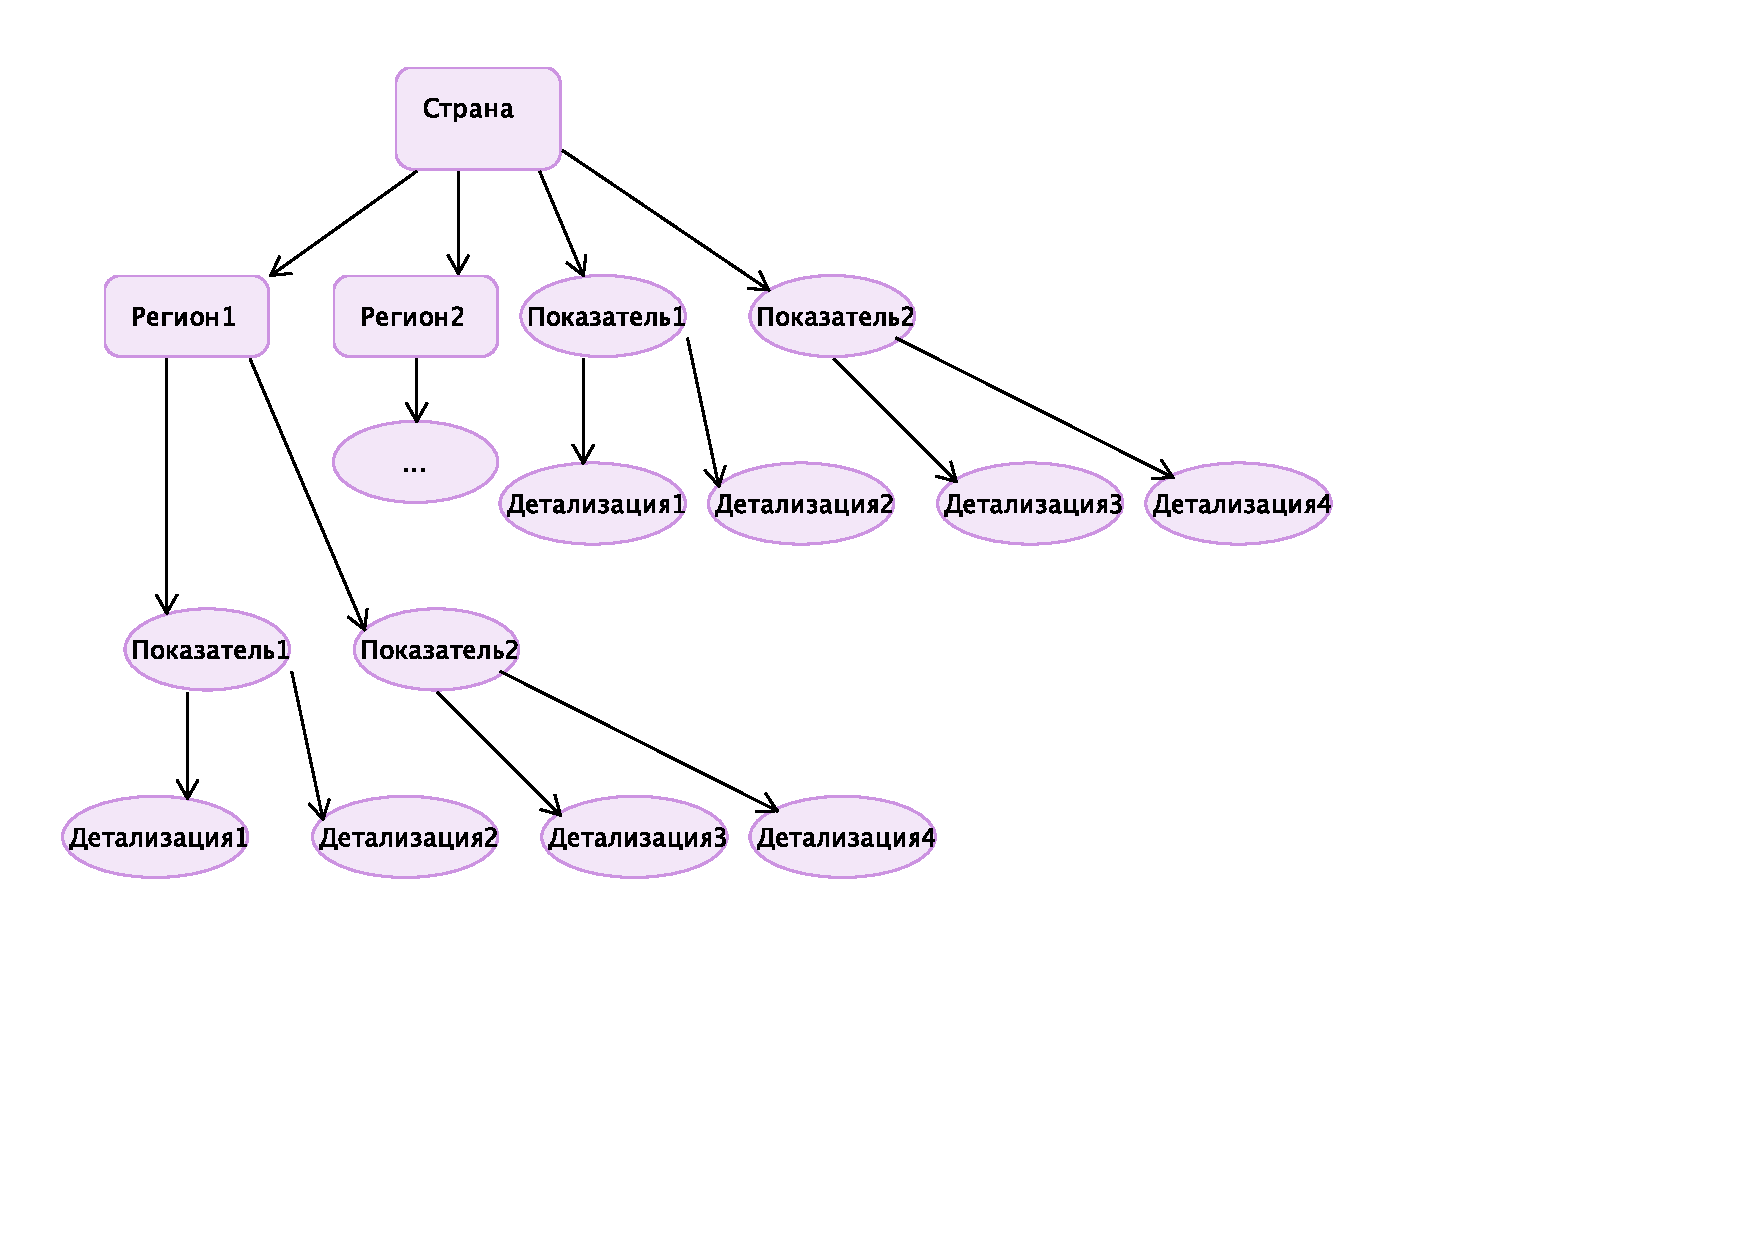
\includegraphics[scale=0.6, trim=0mm 50mm 70mm 0mm, clip]{../resources/uml/ReportScheme.pdf}
\caption{Cхематичная структура отчета}
\label{gr:report:scheme}
\end{center}
\end{figure} 

На схеме (Рис. \ref{gr:report:scheme}) в виде прямоугольников изображены вершины дерева отчетов,
которые не содержат непосредственно значений вычисляемых показателей, а в виде овалов узлы,
для которых эти значения вычислены. Как видно из схемы, отчет может быть построен с детализацией 
по вершинам дерева регионов, кроме того каждый конкретный показатель может быть детализирован
в соответствии с требованиями пользователя.

Отчет должен генерироваться за определенный период, выбранный пользователем, причем он может быть 
разбит на подинтервалы, для каждого из которых должны быть вычислены значения показателей.
Таким образом каждая вершина дерева отчета со значениями должна содержать в себе список 
значений показателя для каждого из подинтервалов.

В общем виде сценарий генерации отчетов для пользователя должет выглядеть следующим образом:
\begin{enumerate}
\item{
  Пользователь открывает страницу с формой генерации отчета. Предполагается две различные страницы
  для отчетов по Live и VOD.
}
\item{
  Пользователь устанавливает параметры отчета на форме и запускает генерацию отчета.
}
\item{
  После того, как процесс генерации отчета завершился, он становится доступен пользователю для просмотра
  или скачивания.
}
\end{enumerate} 

Стоит уточнить, что в рамках настоящей работы условлено, что сгенерированный отчет должен быть доступен 
для пользователя в виде файла формата Excel, в котором построчно выведено дерево отчетов, а значения показателей
для каждого из подинтервалов периода записано в отдельную колонку.

\subsubsection{Форма параметров отчета}
В этом разделе перечислены основные параметры для построения отчета, в том числе специфичные для отчетов
по Live и VOD. Все значения параметров должны сохраняться для каждого пользователя таким образом,
чтобы при возобновлении работы с формой восстанавливались значения последней сессии.

\paragraph{Период отчета} Интервал дат, на основе которого выбирается период, за который строится отчет.
Должна быть возможность задать один из периодов по умолчанию: "За последнюю неделю", "За последний месяц",
"За последний год".

\paragraph{Периодичность данных} Параметр, определяющий способ разбиения выбранного периода на подинтервалы.
Возможные значения: "По дням", "По неделям", "По месяцам", "По кварталам", "По годам".

\paragraph{Валюта} Параметр задает, в каких валютах выводить данные. 
Если параметр не установлен, идет пересчет всех сумм в рубли. 
Если параметр установлен, в отчете в разделе "Отчисления" появляются дополнительные строки: "в т.ч. в долларах", 
"в т.ч. в евро". Одновременно могут быть выбраны несколько значений.

\paragraph{Детализация по территориям} Параметр, определяющий структуру дерева регионов, на основе
которой будет построен отчет

Возможные значения детализации по территориям:
\begin{itemize}
\item{
Регионы, Филиалы, Города
}
\item{
Регионы, филиалы
}
\item{
Филиалы
}
\item{
Регионы
}
\item{
Города
}
\end{itemize}

Также этот параметр определяет диалог выбора значений для параметра “Фильтр по территориям”.

\paragraph{Фильтр по территориям} Определяет, по каким территориям будут показаны данные в отчете. 
Позволяет пользователю выбрать произвольное число регионов.

\paragraph{Правообладатели} Параметр задает фильтр по правообладателям. 
Диалог выбора представляет собой список правообладателей по всем договорам за период отчета, отсортированный в алфавитном порядке.

\paragraph{Показатели} Параметр позволяет пользователю выбрать один или более показателей, для которых будут вычисляться значения.

\paragraph{Детализация по пакетам и телеканалам} \textit{(только для Live)}
Параметр задающий уровни детализации показателей. Возможные значения:
"Без детализации", "По пакетам", "По телеканалам", "По пакетам, затем по телеканалам",
"По телеканалам, затем по пакетам".

\paragraph{Фильтр пакетов и телеканалов} \textit{(только для Live)} Параметры, определяющие для каких именно пакетов
и телеканалов вычисляются значения показателей.

\subsubsection{Описание показателей}
Каждый из описанных ниже показателей должен быть доступен для выбора пользователю при генерации
отчета по Live или VOD, кроме того для каждого из них зафиксирован максимальный уровень детализации,
для которого он может быть расчитан. Следует также отметить, что многие из показателей вычисляются
на основе других показателей.

\paragraph{Live}
\begin{itemize}
\item{
\textit{Количество абонентов на начало периода}. Вычисляется на основе данных, формат которых описан в \ref{stat:live}.
 Максимальная детализация в отчете: территория, пакет, телеканал, дата.
}
\item{
\textit{Количество абонентов на конец периода}. Вычисляется на основе данных, формат которых описан в \ref{stat:live}.
Максимальная детализация в отчете: территория, пакет, телеканал, дата.
}
\item{
\textit{Среднее количество абонентов за период}.  Вычисляется как среднее арифметическое количества абонентов на начало 
и конец периода. Максимальная детализация в отчете: территория, пакет, телеканал, дата.
}
\item{
\textit{Выручка}. Вычисляется на основе данных, формат которых описан в \ref{stat:live}.
Максимальная детализация в отчете – территория, пакет, дата (по телеканалам не считается).
}
\item{
\textit{Отчисления}. Вычисляется на основе данных, формат которых описан в \ref{live:deducts}.
Максимальная детализация в отчете: территория, пакет, телеканал, дата.
}
\item{
\textit{Прибыль} = выручка – отчисления. Максимальная детализация в отчете: территория, пакет, дата (по телеканалам не считается). 
}
\item{
\textit{Маржинальность} = прибыль/выручка*100\%. Максимальная детализация в отчете: территория, пакет, дата (по телеканалам не считается).
}
\item{
\textit{ARPU} = выручка/среднее количество пользователей за период. Максимальная детализация в отчете: территория, пакет, дата (по телеканалам не считается).
}
\end{itemize}

\paragraph{VOD}
\begin{itemize}
\item{
\textit{IPTV Active 30d EOP}. Вычисляется как $\frac{IPTVbase_{end} - IPTVbase_{begin}}{IPTVbase_{begin}} \times 100 \% $, 
где $IPTVbase_{begin}$ и $IPTVbase_{end}$ --- значение IPTV базы за 30 дней на начало и конец периода (см. \ref{stat:live}).
}
\item{
\textit{VOD выручка (без НДС)}. Вычисляется на основе данных, формат которых описан в \ref{stat:vod}, как сумма оплаченных
заказов по VOD.
}
\item{
\textit{VOD выручка (c НДС)}. Вычисляется на основе данных, формат которых описан в \ref{stat:vod}.
}
\item{
\textit{Отчисления}. Cумма отчислений по VOD за период.
}
\item{
\textit{Отчисления по фиксированному платежу (без НДС)}. Уплаченная сумма отчислений по фиксированному платежу за период.
}
\item{
\textit{Отчисления по минимальной гарантии (без НДС)}. Уплаченная сумма отчислений по минимальной гарантии за период.
}
\item{
\textit{Отчисления по разделению дохода (без НДС)}. Уплаченная сумма отчислений по разделению дохода за период.
}
\item{
\textit{Прибыль (без НДС)}. Вычисляется как ``(Выручка по VOD / 1.18) – Отчисления''.
}
\item{
\textit{Маржинальность (без НДС)}. Вычисляется как ``Прибыль по VOD без НДС / выручка по VOD без НДС * 100%``
}
\item{
\textit{Количество заказов}. Сущетсвует три показателя этого типа в зависимости от типа заказов: платный / бесплатный / любой.
}
\item{
\textit{Среднее количество покупок на IPTV пользователя}. Вычисляется как
Количество платных заказов по VOD / Active IPTV Base 30d, причем Active IPTV Users 30d берется на конечную дату периода.
}
\item{
\textit{Количество пользователей}. Вычисляется с помощью подсчета уникальных идентификаторов пользователей из заказов VOD
(см. \ref{stat:vod}). Также как и для Количества заказов существует три показателя этого типа.
}
\item{
\textit{Проникновение пользователей в IPTV}. Вычисляется как 
``Кол-во VOD-пользователей/ Active IPTV 30d Base * 100\%''. Также как и для Количества пользователей существует три показателя этого типа. 
}
\item{
\textit{Средне количество заказов}. Вычисляется как
``Количество заказов VOD /  количество абонентов''. Также как и для Количества пользователей существует три показателя этого типа.
}
\item{
\textit{Средняя стоимость платных заказов VOD (без НДС)}. Вычисляется как 
``(Выручка по VOD / 1.18) / Количество платных заказов за период''.
}
\item{
\textit{ARPU (без НДС) на VOD пользователей}. Вычисляется как ``выручка без НДС / количество уникальных пользователей VOD''
}
\item{
\textit{ARPU (без НДС) на VOD пользователей сделавших платный заказ}. 
Вычисляется как ``выручка без НДС / количество уникальных пользователей VOD, сделавших платный заказ''.
}
\item{
\textit{ARPU (без НДС) на IPTV-пользователей}. Вычисляется как ``выручка без НДС / Active IPTV Base 30d''.
}
\item{
\textit{Количество фильмов, план}.
Количество фильмов, у которых есть ассеты за заданный период.
Проверка “входит ли ассет в заданный период” делается на основе полей “Дата начала”, “Дата окончания” у ассета.
(см. \ref{stat:vod})
}
\item{
\textit{Количество фильмов, факт}.
Количество фильмов, у которых есть ассеты за заданный период.
Проверка “входит ли ассет в заданный период” делается на основе того, есть ли хотя бы 1 заказ на ассет за заданный период.
}
\end{itemize}

\subsection{Авторизация и разграничения прав доступа}
В разрабатываемой системе должны должны быть реализованы механизмы аутентификации и авторизации пользователей
с возможностью разграничения прав доступа к различным модулям системы.

Должны быть предусмотрены следующие сценарии:
\begin{enumerate}
\item{
Просмотр списка пользователей в соответствии с пунктом \ref{crud:list}.
}
\item{
Создание, изменение, удаление пользователей, активация новых пользователей в соответствии с \ref{crud:forms}.
}
\item{
Редактирование собственного профиля пользователя (редактирование логина, пароля, e-mail, имени, фамилии).
}
\item{
Аутентификация, выход из системы.
}
\end{enumerate}

Администратором системы для каждого пользователя может быть выбрано подмножество прав доступа из следующего списка:
\begin{itemize}
\item{
Live. Чтение
}
\item{
Live. Запись
}
\item{
Live. Доступ к коммерческим условиям
}
\item{
Vod. Чтение
}
\item{
Vod. Запись
}
\item{
Vod. Доступ к коммерческим условиям
}
\item{
Системные настройки. Чтение
}
\item{
Системные настройки. Запись
}
\item{
Системные настройки / Пользователи. Чтение
}
\item{
Системные настройки / Пользователи. Запись
}
\end{itemize}

Права на чтение и запись дают доступ на чтение и запись (добавление, изменение удаление записей) для всех форм в соответствующем разделе.

Раздел ``Системные настройки'' содержит страницы справочников, общих для разделов Live и Vod, а также интерфейс для
импорта данных и запуска расчета отчислений по IPTV.

Права на доступ к коммерческим условиям разрешают или запрещают доступ к страницам, на которых упоминаются денежные суммы 
или условия лицензий или договоров. Для таких страниц для чтения должны быть установлены одновременно права на чтение и 
права на доступ к коммерческим условиям, для записи - одновременно установлены право на запись и права на доступ к 
коммерческим условиям. \textit{Исключение: для отчетов, если у пользователя не установлены права доступа к коммерческим условиям, 
но есть право на чтение, то пользователю доступны только параметры отчета и данные отчета, не содержащие коммерческих условий.}

\section{Программная реализация}
В данной главе рассмотрены уже существующие решения, связанные с генерацией отчетов, 
а также детально описана программная реализация полученной в рамках настоящей работы системы.

\subsection{Обзор существующих решений для генерации отчетов}
На данный момент существует множество систем, которые могут использоваться
для автоматической генерации отчетов по уже имеющимся данным: 
среди них есть, как простые, которые предоставляют интерфейс для построения
простых табличных отчетов на основе массива данных (например BandedReportGenerator\cite{BandedReportGenerator}),
так и более комплексные, предоставляющие возможность составления отчетов на основе 
языка RDL (Report Definition Language\cite{rdl_spec}), генерировать OLAP-кубы\cite{olap},
самостоятельно работать с подключением к источнику данных и т.д.

В рамках данного раздела рассмотрены два наиболее популярных программных комплекса
для работы с отчетами: ``SAP Crystal Reports''\cite{crystal_reports} и 
``SQL Server Reporting Services''\cite{sql_reporting} для Microsoft SQL Server, 
оценены их достоинства и недостатки, а также обосновано решение, принятое к реализации.

\subsubsection{SAP Crystal Reports}
\begin{figure}[!ht]
\begin{center}
\hspace*{-1cm} 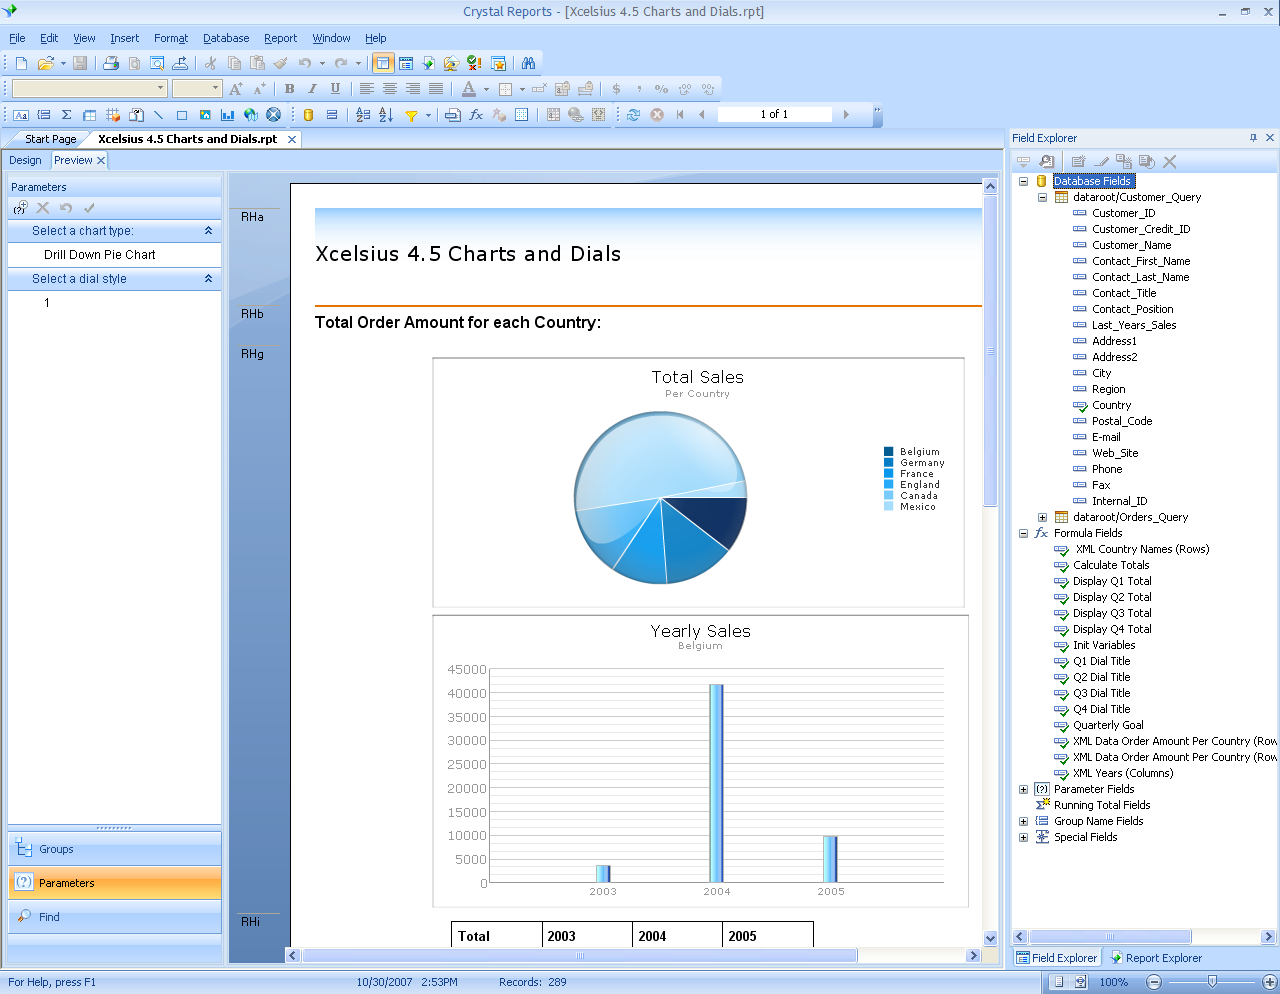
\includegraphics[scale=0.4]{../resources/CrystalReports2008.png}
\caption{Скриншот Crystal Reports 2008}
\label{gr:crystal_screenshot}
\end{center}
\end{figure}

\textit{Crystal Reports} является наиболее популярным продуктом компании SAP, состоит из
множества приложений таких как ``Crystal Reports Server'', ``Crystal Reports Viewer'',
``Crystal Reports Designer'', а так же плагина для Microsoft Visual Studio, позволяющего
составлять шаблоны отчетов в среде разработки.
 
\paragraph{Достоинства}
\begin{itemize}
\item{
Простой интерфейс для построения несложных отчетов.
}
\item{
Возможность генерации OLAP-кубов\cite{olap}, удобное представление
древообразной структуры отчета, описанной в \ref{section:stat_reports_task}.
}
\item{
Реализована работа с базой данных.
}
\item{
Реализована возможность графической интерпретации отчетов.
}
\end{itemize}

\paragraph{Недостатки}
\begin{itemize}
\item{
Отсутствие готовых решений для генерации отчетов через веб-интерфейс.
}
\item{
Недостаточная гибкость вычисления показателей, ограниченная пользовательскими формулами.
}
\item{
Инкапсуляция методов обработки данных, ограничивающая возможность оптимизировать
запросы к СУБД.
}
\end{itemize}

\subsubsection{SQL Server Reporting Services}
\begin{figure}[!ht]
\begin{center}
\hspace*{-1cm} 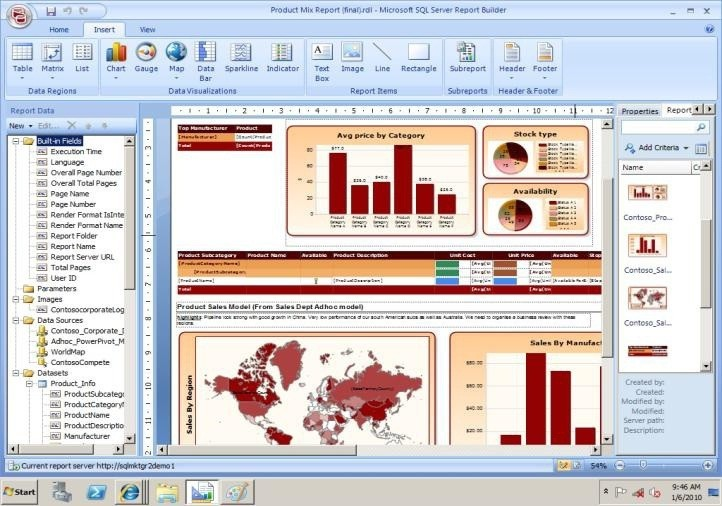
\includegraphics[scale=0.7]{../resources/SQLReporting.jpg}
\caption{Скриншот приложения Microsoft SQL Server Reporting Services 2008}
\label{gr:crystal_screenshot}
\end{center}
\end{figure}
Комплекс приложений \textit{SQL Server Reporting Services} создавался как конкурент для
\textit{SAP Crystal Reports}. В нем реализованы по сути те же базовые инструменты для конструирования
и просмотра отчетов, но при этом добавлены некоторые элементы функциональности, 
позволяющие Reporing Services занимать достойную позицию на рынке Business Intellegence технологий.

\paragraph{Достоинства}
\begin{itemize}
\item{
Более тесная интеграция с СУБД Microsoft SQL Server, которая в соответствии 
с нефункциональными требованиями к системе (см. \ref{part:requirements}) должна быть
использована в качестве хранилища данных.
}
\item{
Реализованы модули просмотра отчетов для ASP.NET\cite{sql_reporting}, что позволяет
реализовать генератор в виде веб-приложения.
}
\item{
Язык RDL\cite{rdl_spec}, реализованный на основе XML, позволяет специфицировать вид шаблона отчета,
на основе которого может быть сгенерирован отчет для пользователя, как через 
веб-интерфейс, так и с использованием Desktop-приложения.
}
\end{itemize}

\paragraph{Недостатки} В SQL Reporting Services присутствуют те же недостатки, что и в случае
с Crystal Reports, за исключением возможности генерации отчетов через веб-интерфейс.

\subsubsection{Результаты обзора}
Оба рассмотренные в предыдущих разделах программных продукта 
обладают неоспоримыми достоинствами, предлагая, как конечному пользователю, так и разработчику,
большой диапазон инструментов, позволяющих решать самый широкий круг задач.
Однако на первом этапе реализации системы было принято решение избежать их использования
в связи с серьезными рисками, возникающими в случае их применения в связи с
высокой степенью инкапсуляции механизмов построения отчетов в этих системах.

Возможные проблемы, вызванные инкапсуляцией включают:
\begin{itemize}
\item{
Невозможность достаточно тонкой настройки генератора может привести к несоответствиям в результате
работы генератора отчетов и требований к ним.
}
\item{
Невозможность оптимизации запросов к СУБД. Это может привести к тому, что при большом количестве данных
время генерации отчетов будет выходить за рамки, оговоренные в требованиях.
}
\end{itemize}

Таким образом в рамках данной работы было необходимо разработать оригинальный 
алгоритм генерации отчетов, результат работы которого должен удовлетворять требованиям,
описанным в первой главе.

При этом, учитывая факт использования в системе Microsoft SQL Server, не стоит исключать
возможность генерации более простых отчетов с помощью SQL Reporting Services, которое
пользователь сможеть осуществить самостоятельно при наличии доступа к серверу СУБД.




\newpage
\newpage
%%\section*{Заключение}
\addcontentsline{toc}{section}{\hspace{7mm}Заключение}

По~результатам выполненной работы сделаны следующие выводы:

\begin{enumerate}
\item {
Автором была спроектирована и реализована в виде миграций схема
Базы данных.
}
\item {
Спроектирован и реализован механизм запуска фоновых задач для веб-приложений, написанных
на языке программирования PHP.
}
\item {
Разработан модуль для расчета отчислений по категори Live, а также соответствующий
пользовательский интерфейс. 
}
\item {
Спроектирован и реализован пользовательский интерфейс для поиска
и редактирования данных (для более чем 20 множеств сущностей).
}
\item {
Проведены исследование и условная классификация существующих 
решений для генерации отчетов. 
Проанализированы и показаны достоинства и недостатки исследованных решений.
}
\item {
Автором разработан модуль генерации отчетов и реализован
пользовательский интерфейс для генерации статистических отчетов
по категориями Live и VOD.
}
\end{enumerate}

В~ходе следующих этапов разработки планируется:
\begin{enumerate}
\item {
Реализовать интерпретацию отчетов в виде графиков и диаграмм.
}
\item {
Разработать интерфейс для просмотра отчета в процессе генерации.
}
\item {
Оптимизировать процесс генерации отчетов за счет уменьшения количества избыточных данных.
}
\end{enumerate}

\newpage

\addcontentsline{toc}{section}{\hspace{7mm}Список литературы}
\begin{thebibliography}{0}
\bibitem{BandedReportGenerator}
Banded Report Generator. --- \url{http://smarty.incutio.com/?page=BandedReportGenerator}

\bibitem{rdl_spec}
Report Definition Language Specification. --- \url{http://msdn.microsoft.com/en-us/library/dd297486.aspx}

\bibitem{olap}
Wrembel,~R.~
Data Warehouses and OLAP: Concepts, Architectures and Solutions./
Robert Wrembel, Christian Koncilia //
2007. IRM~Press.

\bibitem{crystal_reports}
SAP~Crystal~Reports. --- \url{http://www.crystalreports.com/}

\bibitem{sql_reporting}
SQL~Server~Reporting~Services. --- \url{http://www.microsoft.com/en-us/sqlserver/solutions-technologies/business-intelligence/reporting.aspx}



\end{thebibliography}
\newpage

\begin{center}
Приложение
\end{center}
\addcontentsline{toc}{section}{\hspace{7mm}Приложение}
%\appendix

\section{Справка о внедрении результатов ВКР}
\begin{figure}[!ht]
\begin{center}
\hspace*{-1cm} 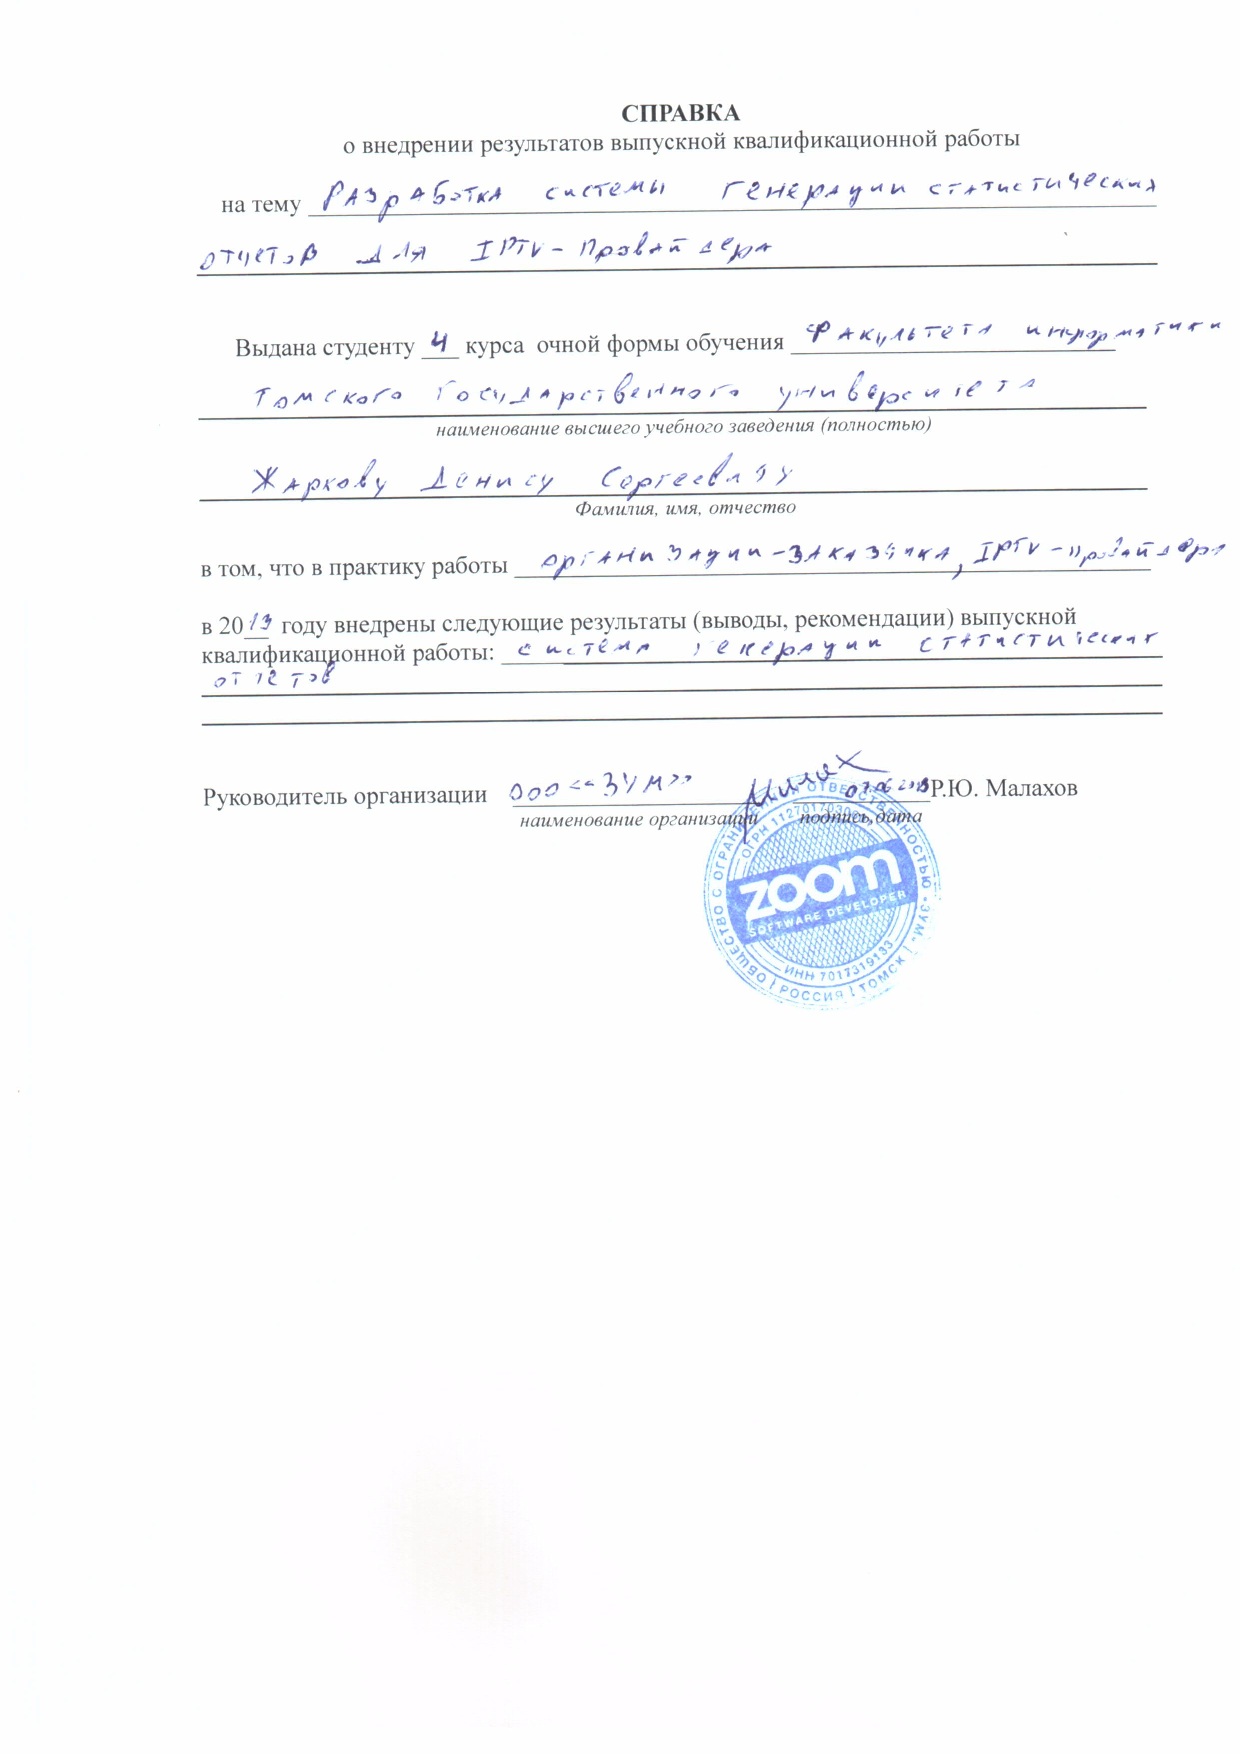
\includegraphics[scale=1, trim=30mm 120mm 0mm 10mm, clip]{../resources/inquiry.pdf}
\end{center}
\end{figure}

\newpage


\section{Руководство пользователя}

Для использования системы необходимо:
\begin{itemize}
\item{
 Чтобы она была установлена и настроена в соответствии с Руководством администратора.
}
\item{
 Веб-сервер доступен по сети из рабочей станции пользователя.
}
\item{
 На рабочей станции пользователя установлен один из веб-браузеров: 
Internet Explorer (версия >= 7), Google Chrome (версия >= 15.0), Firefox (версия >= 3.0).
}
\end{itemize}


\subsection*{Начало работы}

В начале работы пользователь вводит в адресную строку браузера URL-адрес веб-сервера.
В случае, если сессия не была инициализирована, будет открыта страница входа.

Предполагается, что пользователь знаком с предметной областью IPTV услуг.

\begin{figure}[!ht]
\begin{center}
\hspace*{-1cm} 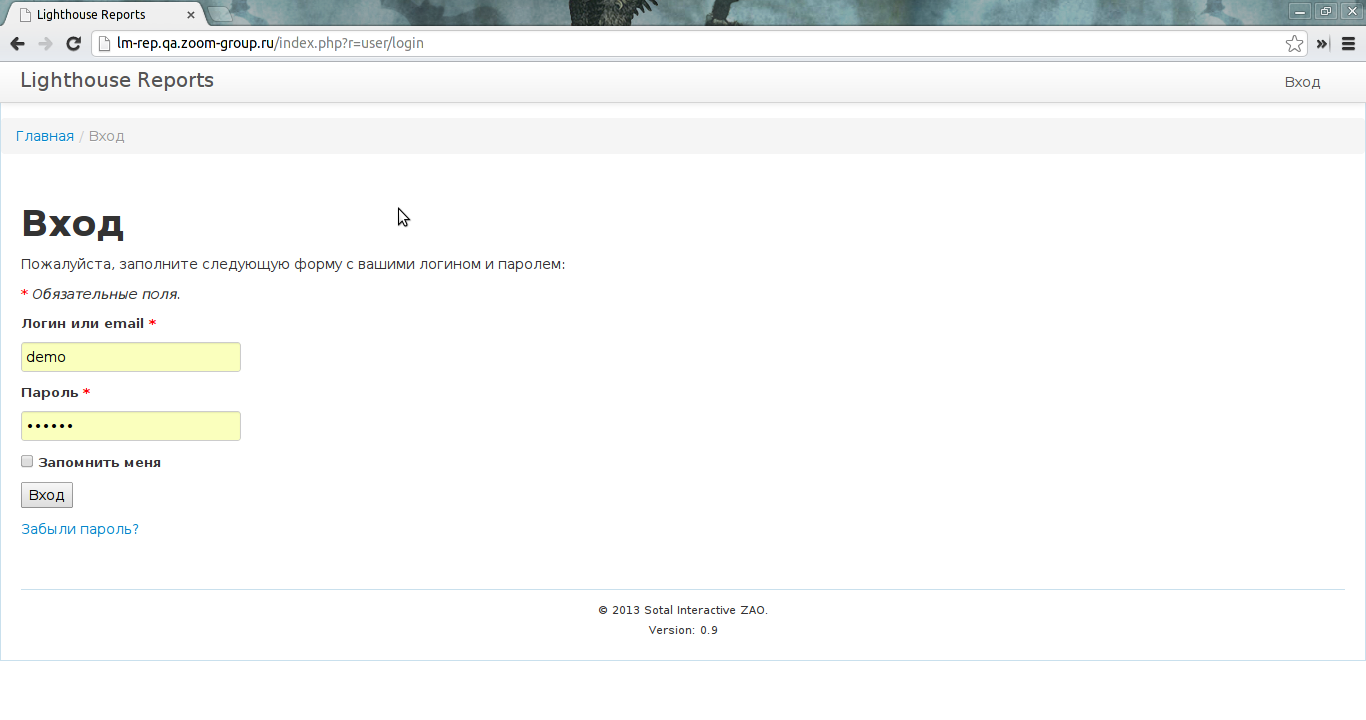
\includegraphics[scale=0.35, trim=0mm 0mm 0mm 10mm, clip]{../resources/screens/login.png}
\end{center}
\end{figure}

\begin{figure}[!ht]
\begin{center}
\hspace*{-1cm} 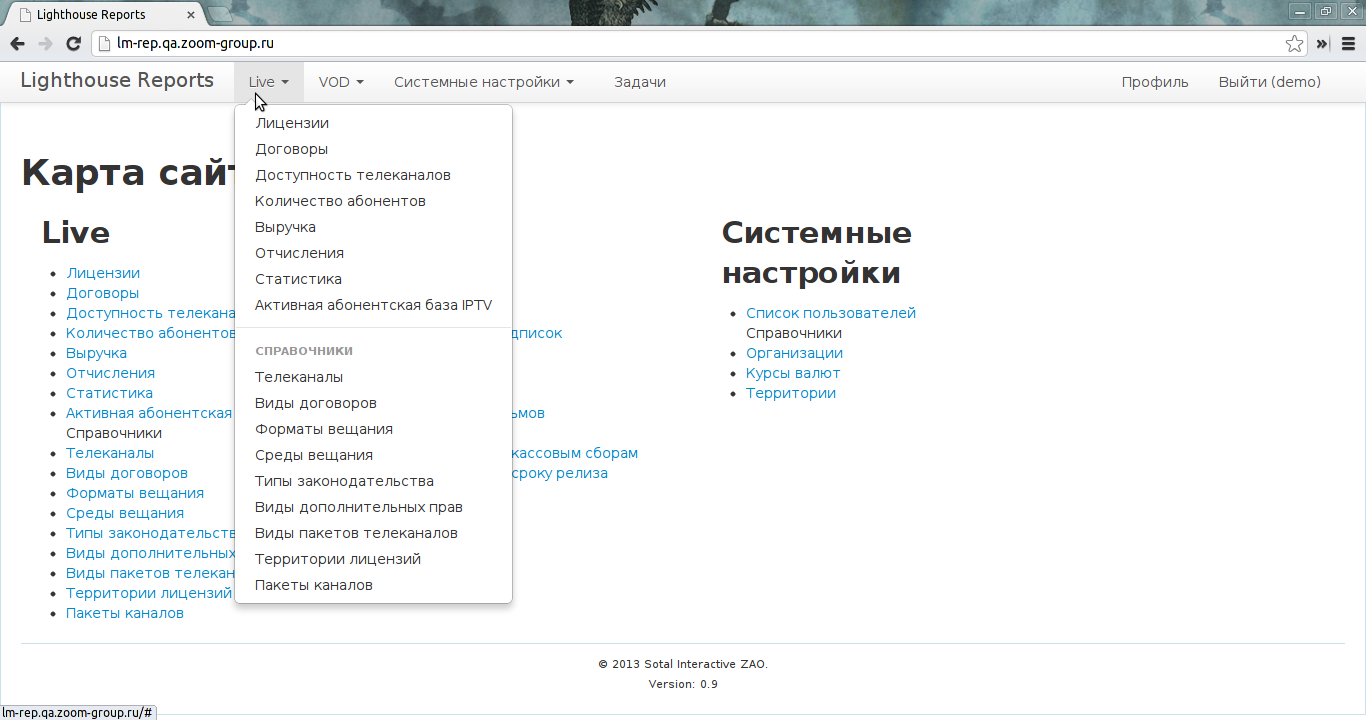
\includegraphics[scale=0.28, trim=0mm 0mm 0mm 10mm, clip]{../resources/screens/map.png}
\end{center}
\end{figure}

\vspace*{-1cm} 

После ввода правильных аутентификационных реквизитов, открывается Карта сайта --- раздел системы, в котором
выведены все доступные пользователю разделы системы. Кроме карты сайта, доступные разделы
также расположены в Главном меню.

Приложение состоит из трех разделов: Live, VOD и Системные настройки.

\subsection*{Работа с данными}

Большая часть ссылок из подразделов предоставляют интерфейс для поиска/редактирования данных
определенного вида (примеры на рисунках).

\begin{figure}[!ht]
\begin{center}
\hspace*{-1cm} 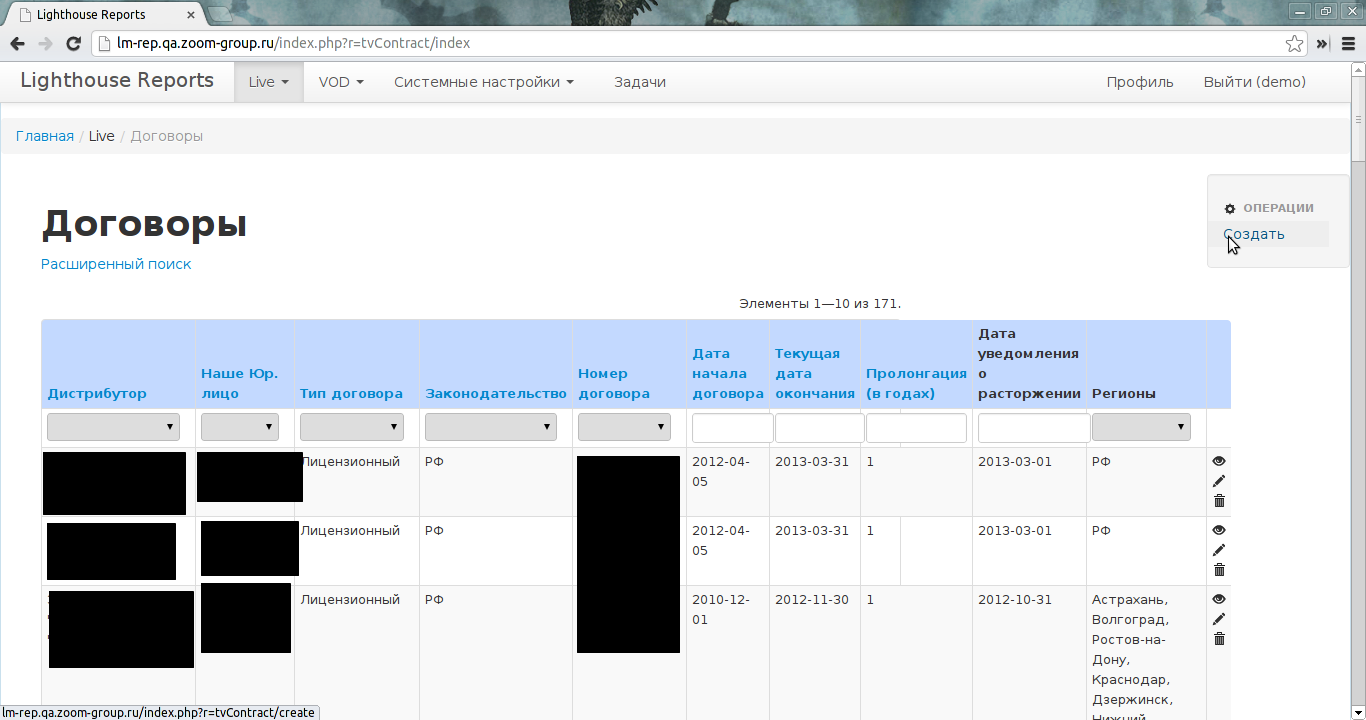
\includegraphics[scale=0.35, trim=0mm 0mm 0mm 10mm, clip]{../resources/screens/contracts.png}
\caption{Главная страница подраздела Live -> Договоры}
\end{center}
\end{figure}

\begin{figure}[!ht]
\begin{center}
\hspace*{-1cm} 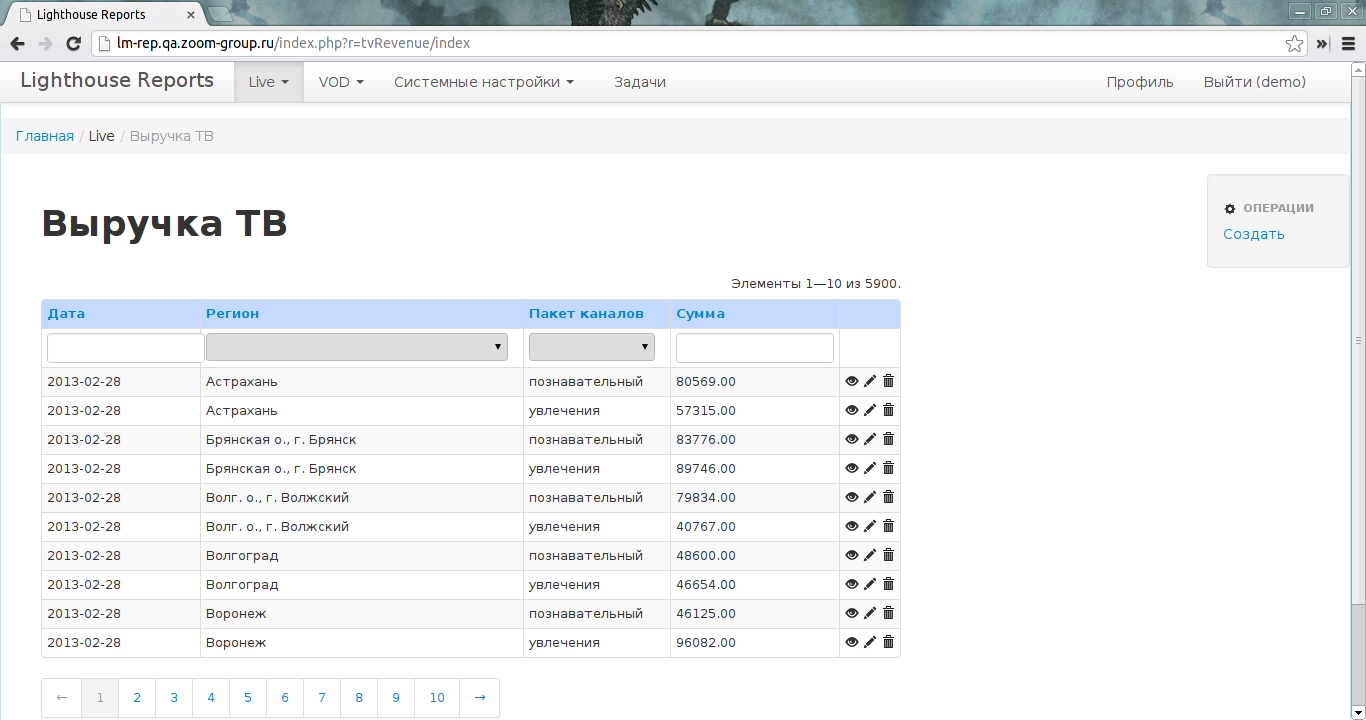
\includegraphics[scale=0.35, trim=0mm 0mm 0mm 10mm, clip]{../resources/screens/tv_revenue.png}
\caption{Главная страница подраздела Live -> Выручка ТВ}
\end{center}
\end{figure}

\begin{figure}[!ht]
\begin{center}
\hspace*{-1cm} 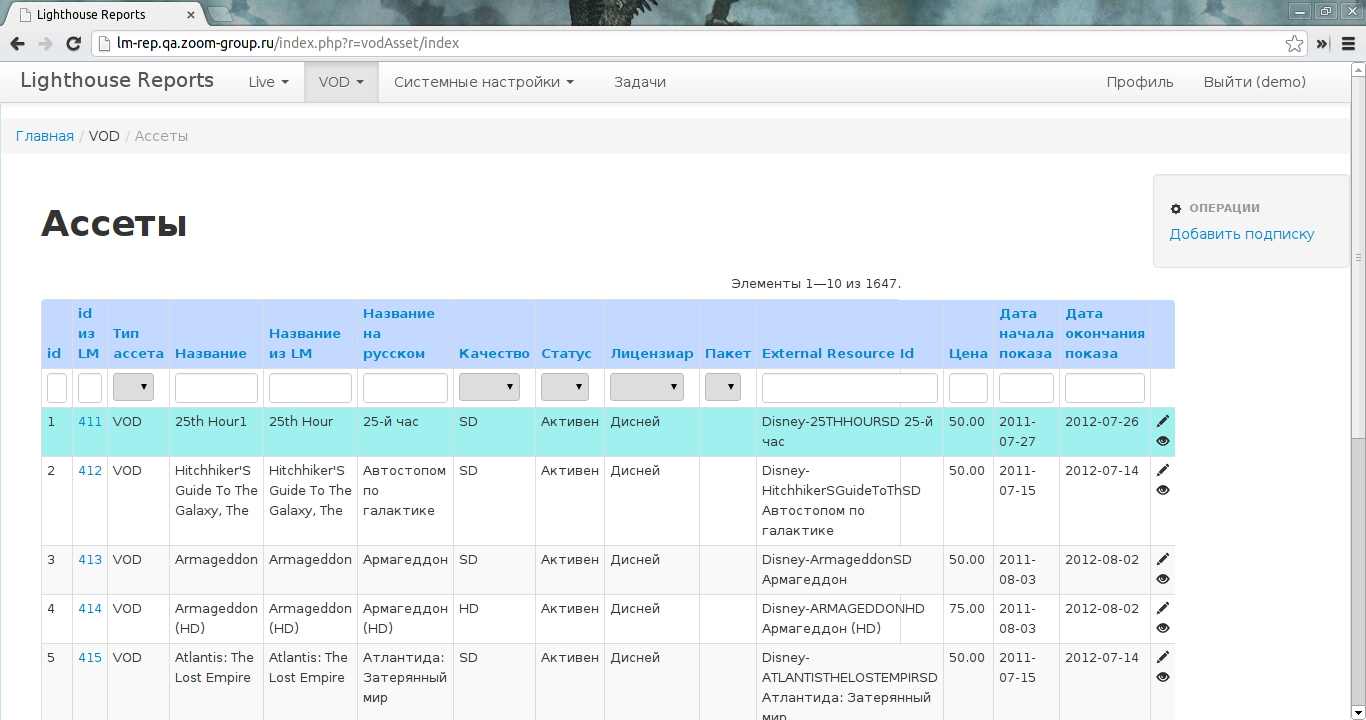
\includegraphics[scale=0.35, trim=0mm 0mm 0mm 10mm, clip]{../resources/screens/assets.png}
\caption{Главная страница подраздела VOD -> Ассеты}
\end{center}
\end{figure}

Находясь на главной странице такого интерфейса, пользователю доступен список объектов в виде таблицы.

Для фильтрации по значению нужно ввести необходимо ввести ключевое слово над соответствующим столбцом,
после чего произойдет обновление содержимого.

Для указания поля сортировки необходимо кликнуть по тексту заголовка соответсвующего столбца. 
Повторные нажатия изменят порядок сортировки или вернут сортировку по умолчанию.

В большинстве подобных интерфейсов присутствуют дополнительные операции, такие как например добавление объекта
(на рисунках в правом верхнем углу).

Для просмотра отдельного объекта нужно кликнуть по иконке с глазом в соответствующей строке.

Для редактирования объекта необходимо нажать на иконку с изображением карандаша, после этого браузер пользователя
перенаправляется на страницу редактирования.

\begin{figure}[!ht]
\begin{center}
\hspace*{-1cm} 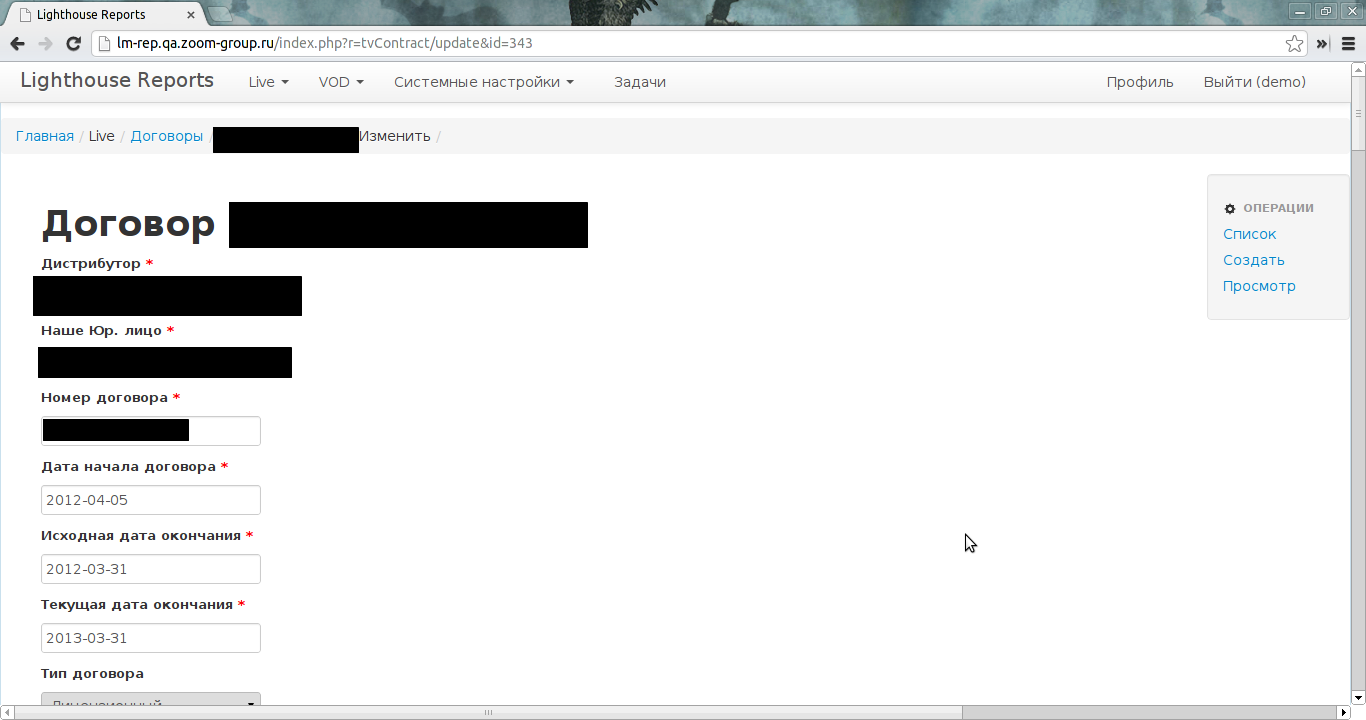
\includegraphics[scale=0.35, trim=0mm 0mm 120mm 10mm, clip]{../resources/screens/contract_edit.png}
\caption{Страница редактирования подраздела Live -> Договоры}
\end{center}
\end{figure}

\begin{figure}[!ht]
\begin{center}
\hspace*{-1cm} 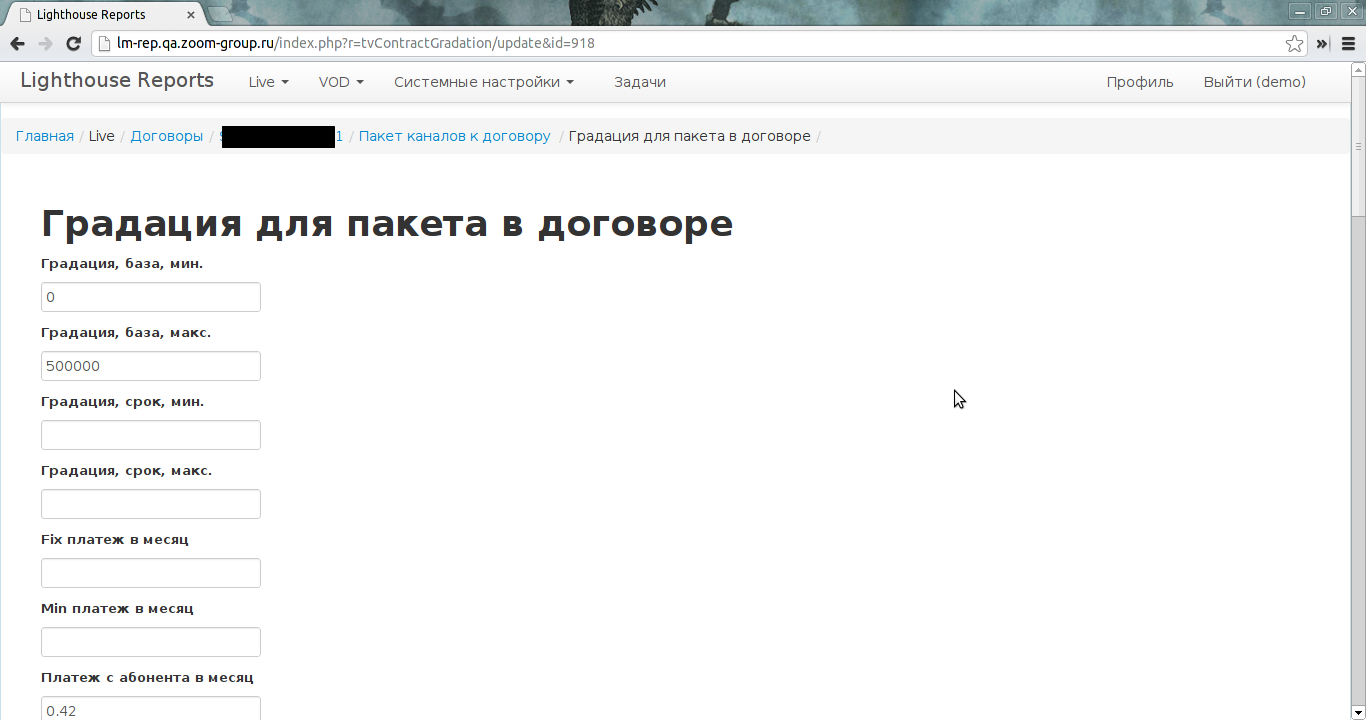
\includegraphics[scale=0.35, trim=0mm 0mm 120mm 10mm, clip]{../resources/screens/contract_gradation.png}
\caption{Страница редактирования градации по договору Live}
\end{center}
\end{figure}

На страницах с формами для редактирования/добавления объектов пользователь может заполнить
необходимые поля и сохранить объект, нажав кнопку "Сохранить" в нижней части страницы.

\begin{figure}[!ht]
\begin{center}
\hspace*{-1cm} 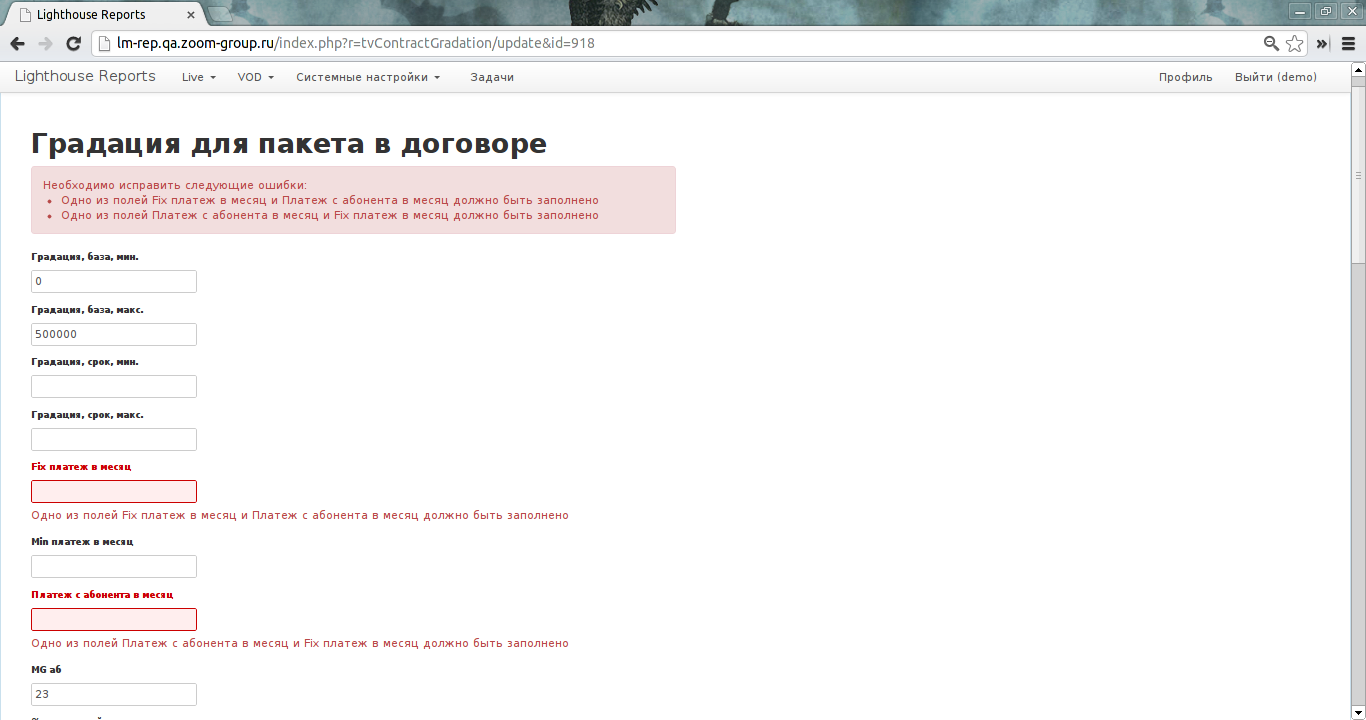
\includegraphics[scale=0.35, trim=0mm 0mm 120mm 10mm, clip]{../resources/screens/contract_gradation_error.png}
\caption{Страница редактирования градации по договору Live. Ошибка}
\end{center}
\end{figure}

В случае если данные формы были заполнены некорректно, объекты не сохраняются,
пользователю выводится уведомление в верхней части страницы. 
Кроме того поля с ошибочными значениями подсвечиваются красным цветом.

\subsection*{Задачи}

\begin{figure}[!ht]
\begin{center}
\hspace*{-1cm} 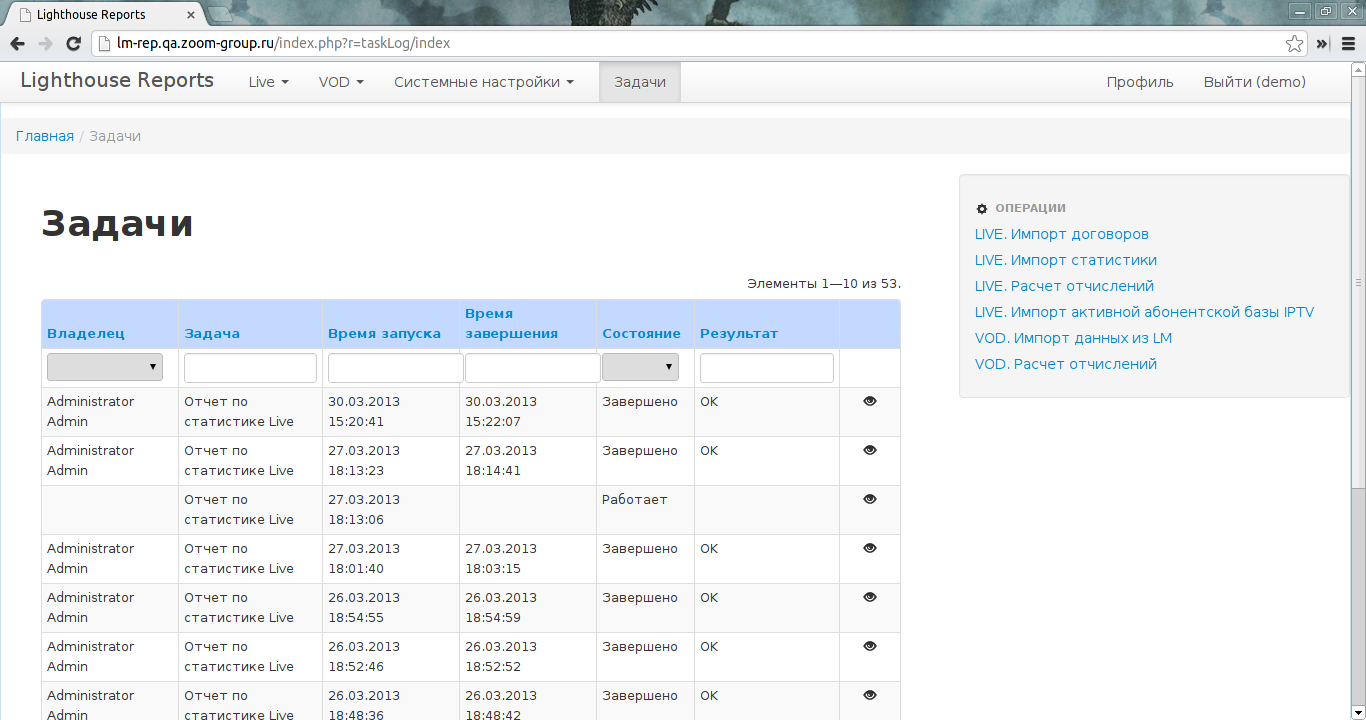
\includegraphics[scale=0.35, trim=0mm 0mm 0mm 10mm, clip]{../resources/screens/tasks.png}
\caption{Раздел задачи}
\end{center}
\end{figure}

В разделе "Задачи" пользователь может отслеживать статус запущенных им фоновых задач
и инициировать запуск новых.

Для просмотра результата завершенной задачи нужно кликнуть по пиктограмме с изображением глаза,
в случае, если результатом работы задачи был файл, он доступен для скачивания.

Для запуска доступны следующие задачи:
\begin{itemize}
\item{
  Импорт договоров по Live из файла в формате Microsoft Excel
}
\item{
  Импорт статистических данных по Live из файла в формате XML
}
\item{
  Расчет отчислений по Live
}
\item{
  Импорт активной абонентской базы из файла в формате Microsoft Excel
}
\item{
  Импорт данных для VOD 
}
\item{
  Расчет отчислений по VOD
}
\end{itemize}

\begin{figure}[!ht]
\begin{center}
\hspace*{-1cm} 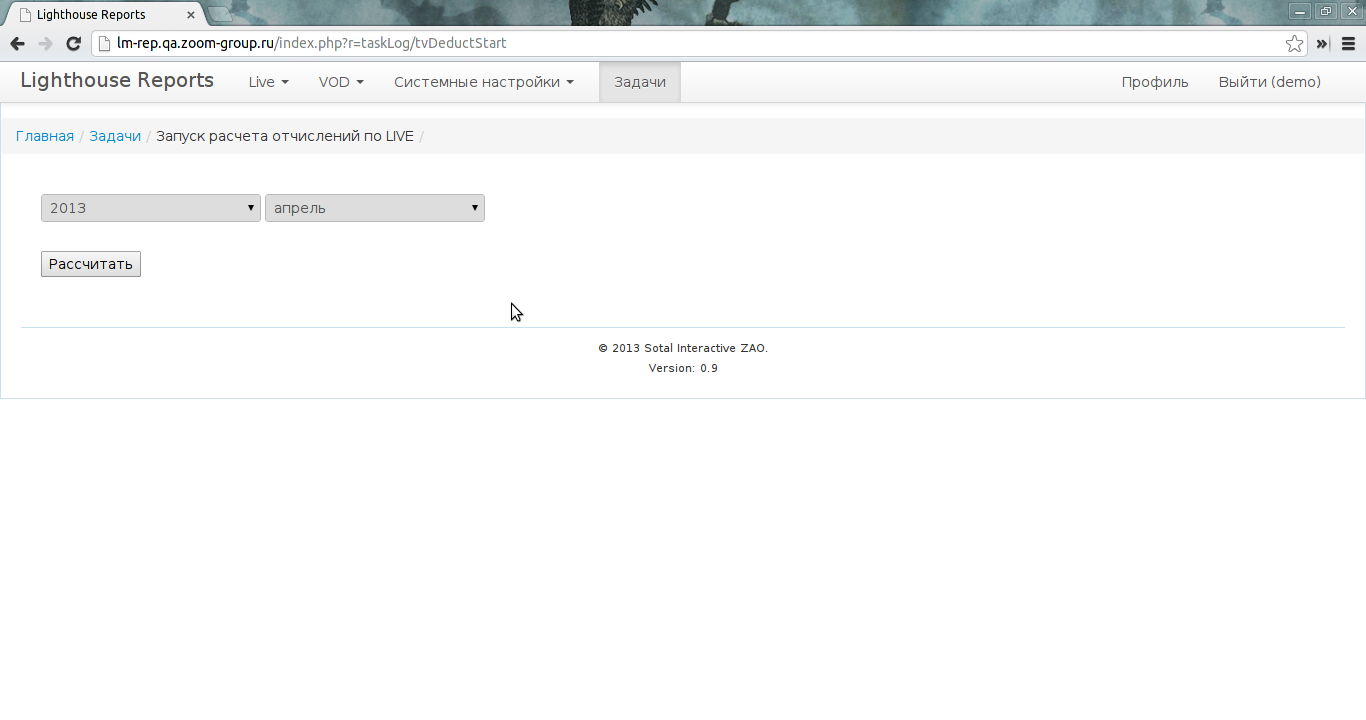
\includegraphics[scale=0.35, trim=0mm 70mm 250mm 10mm, clip]{../resources/screens/deduct_start.png}
\caption{Интерфейс запуска для расчета отчислений по Live}
\end{center}
\end{figure}

\subsection*{Генерация отчетов}
Для работы со статистическими отчетами по Live или VOD необходимы выбрать
в соответствующем разделе меню пункт ``Статистика'', после чего пользователю
становится доступна форма параметров отчета.

Выбранные в форме параметры сохраняются для данного пользователя и могут быть
доступны в рамках последующих сессий использования.

\begin{figure}[!ht]
\begin{center}
\hspace*{-1cm} 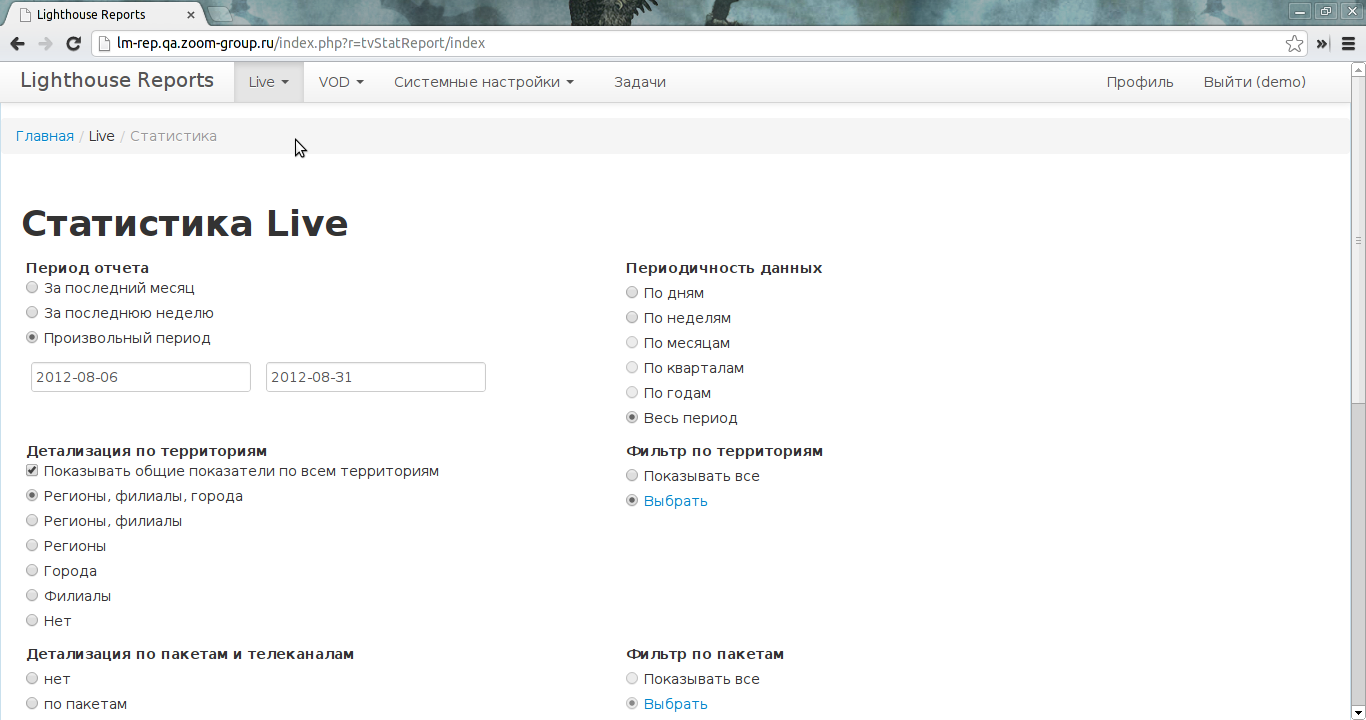
\includegraphics[scale=0.35, trim=0mm 0mm 180mm 10mm, clip]{../resources/screens/live_stat.png}
\caption{Страница Live / Статистика}
\end{center}
\end{figure}

\begin{figure}[!ht]
\begin{center}
\hspace*{-1cm} 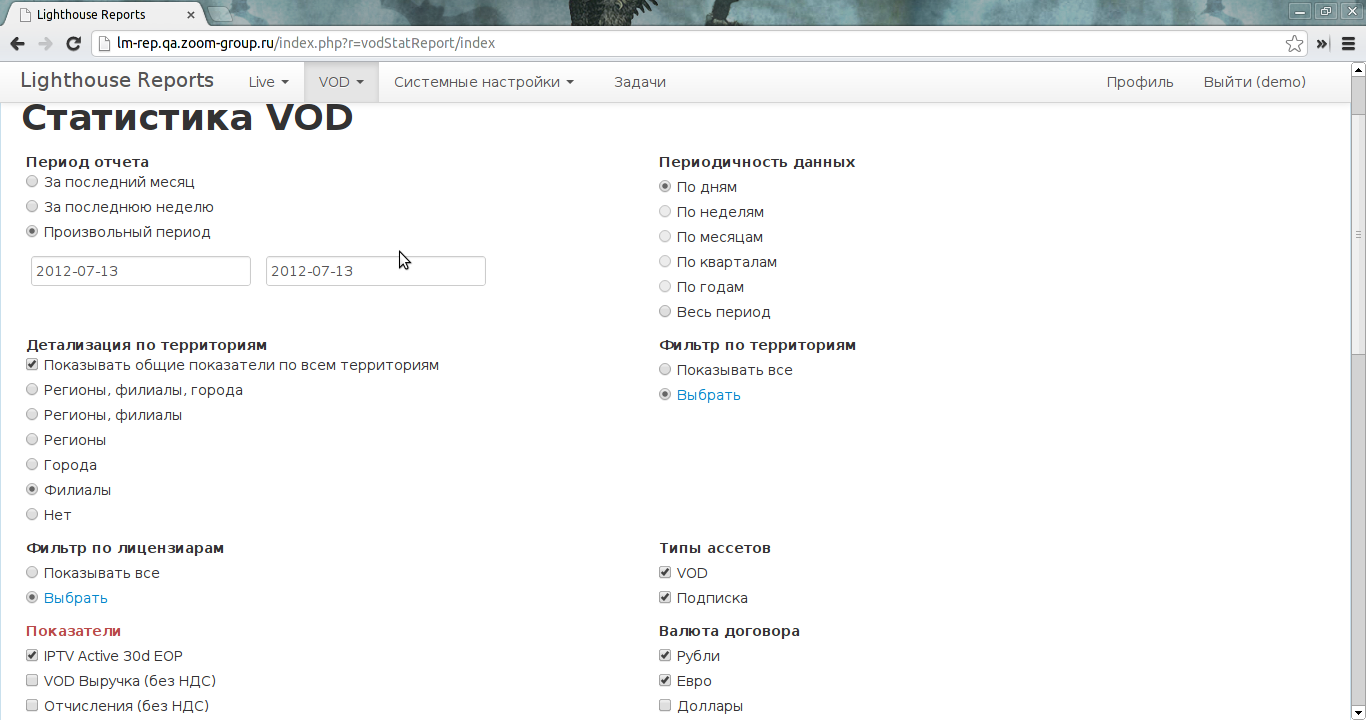
\includegraphics[scale=0.35, trim=0mm 0mm 180mm 10mm, clip]{../resources/screens/vod_stat.png}
\caption{Страница VOD / Статистика}
\end{center}
\end{figure}

\paragraph{Период}
Пользователь может выбрать период отчета из фиксированных вариантов: ``За прошлую неделю''/``За прошлый год''
или указать произвольный интервал дат в полях под надписью ``Произвольный период''.
При нажатии на поле с датой становится доступен вспомогательный элемент с календарем, где может быть
выбран определенный день месяца.

В разделе ``Периодичность данных'' определяется, каким образом выбранный период будет разбиваться на подинтервалы,
для каждого из которых будут вычислены значения показателей.
Варианты разбиения указаны на рисунке и комментариях не нуждаются.

\paragraph{Территории}
Для определения детализации по территориям необходимо выбрать один из пунктов
переключателя в соответствующем разделе страницы формы.
В случае, если отмечен флажок ``Показывать общие показатели по всем территориям'',
то независимо от типа детализации, будут вычислены значения суммарно по всем
территориям (РФ). 

``Фильтр по территориям'' определяет множество регионов, которые будут 
выведены в отчете. При выборе пункта ``Выбрать'' во всплывающем окне будет выведено дерево
территорий в соответствии с текущим типом детализации, где для каждого 
региона, который необходимо вывести должен быть установлен флажок.
В верхней части всплывающего окна доступны кнопки ``Выбрать все'', ``Очистить выбор''.

\begin{figure}[!ht]
\begin{center}
\hspace*{-1cm} 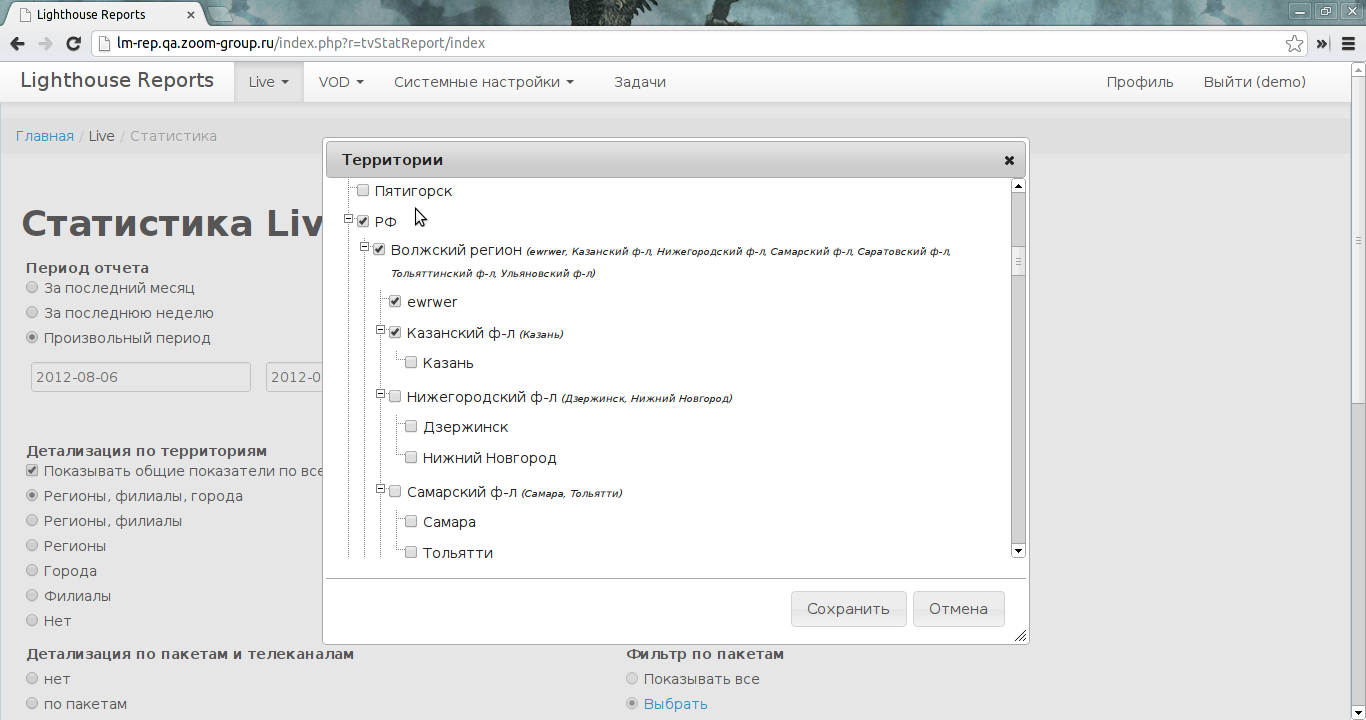
\includegraphics[scale=0.35, trim=0mm 0mm 100mm 10mm, clip]{../resources/screens/live_stat_regions.png}
\caption{Страница Live / Статистика. Фильтр регионов}
\end{center}
\end{figure}

\paragraph{Пакеты и телеканалы}
Функциональность по выбору детализации по пакетам и телеканалам в целом аналогична 
выбору детализации по территориям. Сначала пользователь выбирает один из уровней детализации:
\begin{itemize}
\item{
  Без детализации
}
\item{
  По пакетам
}
\item{
  По телеканалам
}
\item{
  По пакетам, затем по телеканалам
}
\item{
  По телеканалам, затем по пакетам
}
\end{itemize}

После этого в соответствующих фильтрах выбираются пакеты и телеканалы, 
данные по которым должны быть включены в отчет.

\paragraph{Выбор показателей}
В нижней части формы расположен раздел для выбора показателей,
необходимых для вычислений в рамках текущего отчета.
Выбранные показатели отмечаются флажками.

\begin{figure}[!ht]
\begin{center}
\hspace*{-1cm} 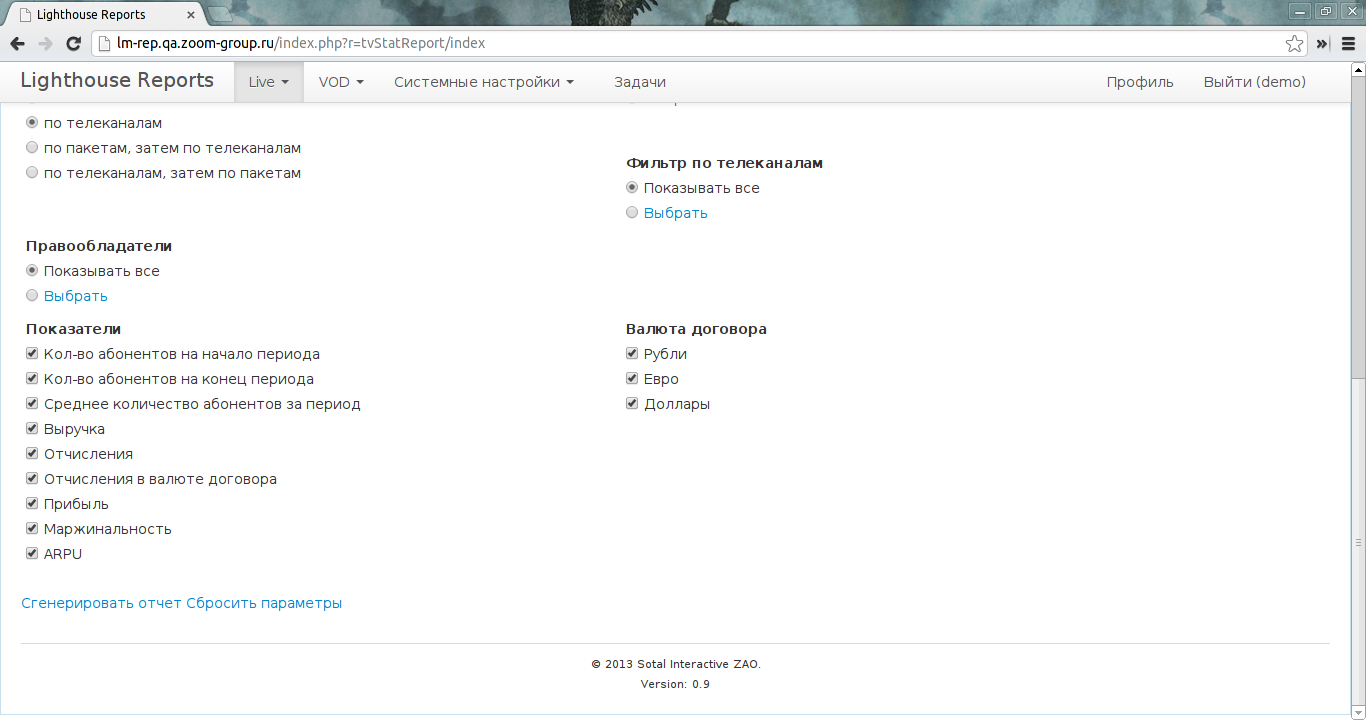
\includegraphics[scale=0.35, trim=0mm 0mm 100mm 10mm, clip]{../resources/screens/live_stat_indicators.png}
\caption{Страница Live / Статистика. Выбор показателей}
\end{center}
\end{figure}

\paragraph{Создание отчета}
После установки параметров пользователь может запустить процесс
генерации отчета, кликнув по кнопке "Сгенерировать отчет".
После этого браузер пользователя перенаправляется на страницу ожидания,
где будет выведен статус выполнения задачи. После окончания процесса
будет инициализировано скачивание файла с отчетом в формате Microsoft Excel.

\begin{figure}[!ht]
\begin{center}
\hspace*{-1cm} 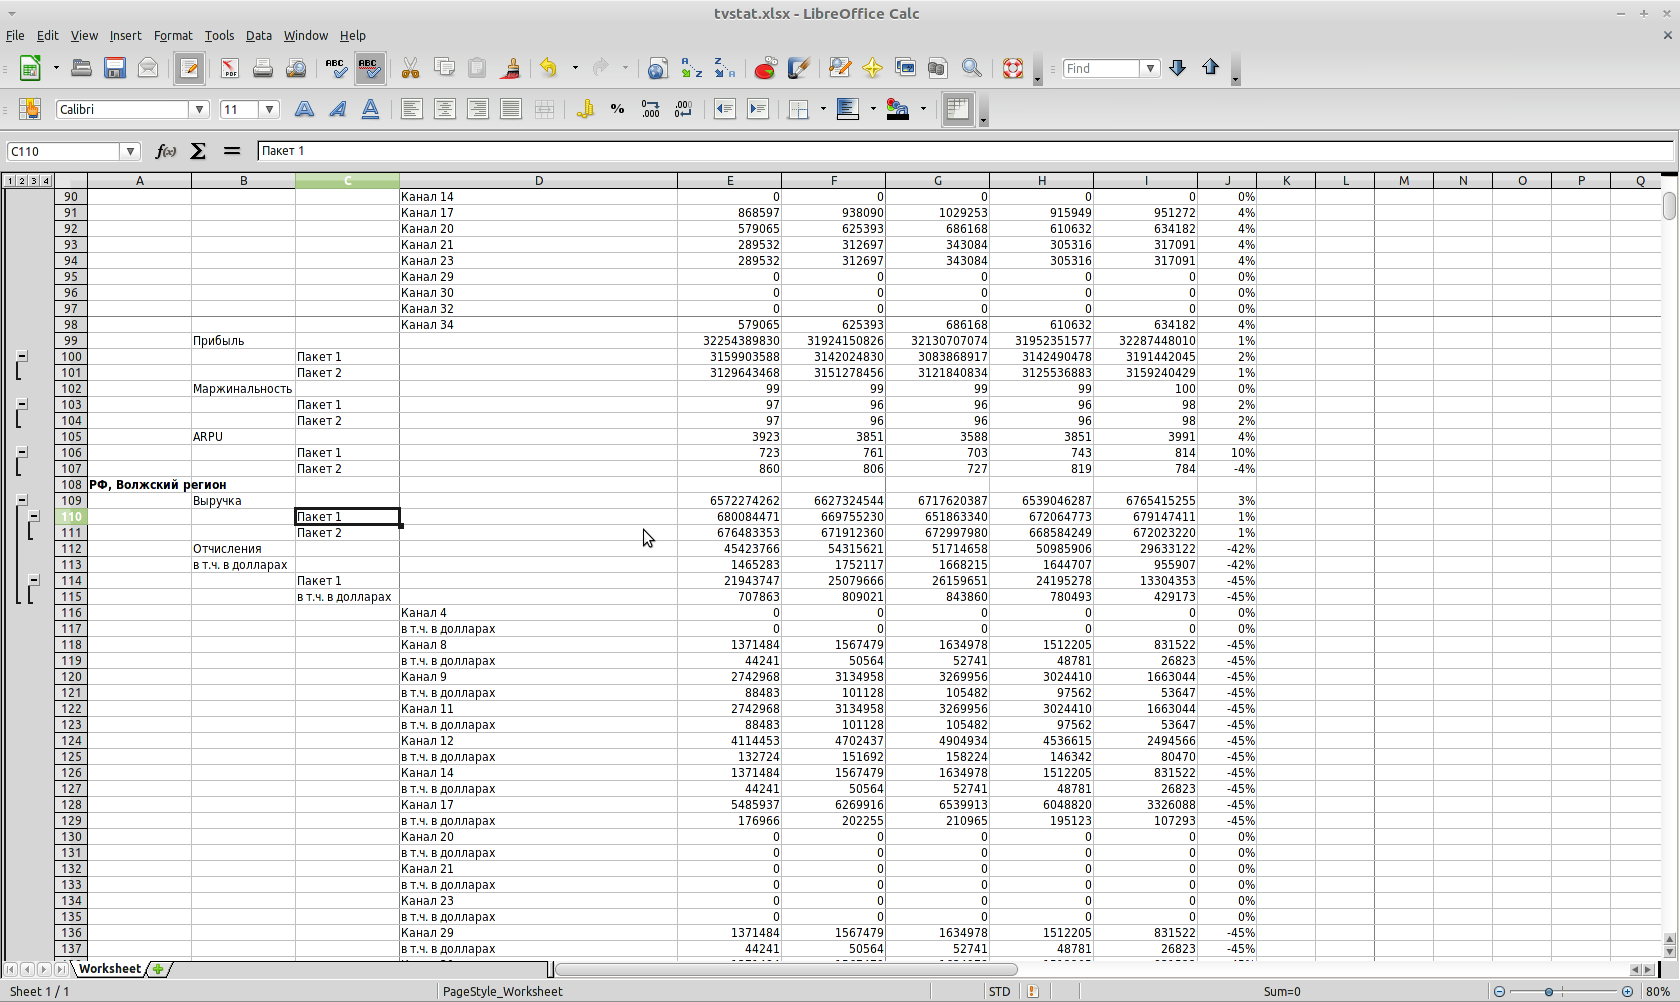
\includegraphics[scale=0.35, trim=0mm 100mm 150mm 50mm, clip]{../resources/report1.png}
\caption{Содержимое файла отчета}
\end{center}
\end{figure}

\paragraph{Структура отчетов}
Файл отчета представляет собой таблицу Excel, первые
столбцы описывают уровни детализации. В последующих столбцах
расположены значения показателей для каждого подинтервала, заключающий столбец
содержит значение End Of Percent показателя.



\newpage
\section{Руководство администратора}

\subsection*{Требования к аппаратному и программному обеспечению}

\textbf{Сервер баз данных:}
\begin{itemize}
\item{
Процессор: XEON, не менее 2х ядер
}
\item{
ОЗУ:  8-16GB
}
\item{
Диск от 250GB
}
\item{
Microsoft Windows Server 2008 Standard (64-bit) 6.0.6002 Service Pack 2 Build 6002 
}
\item{
Microsoft SQL Server Standard Edition (64-bit)
}
\end{itemize}


\textbf{Веб-сервер:}
\begin{itemize}
\item{
Процессор: XEON, не менее 2х ядер
}
\item{
ОЗУ:  4-16GB
}
\item{
Диск от 250GB
}
\item{
rhel-server-6.2-x86\_64
}
\end{itemize}

\textbf{Сеть:} 100Mb соединение между веб-сервером и сервером баз данных.

\subsection*{Установка и настройка системы на Red Hat Enterprise Linux Server 6.2}

Процесс установки системы тестировался на rhel-server-6.2-x86\_64.

В процессе установки сервер должен быть подключен к интернету для загрузки необходимых пакетов.

В описании процесса установки курсивом выделены команды, которые необходимо выполнить в консоли.

Команды необходимо выполнять от имени пользователя, обладающего административными привилегиями.

В случае ошибок при выполнении команд необходимо прервать процесс установки и обратиться к разработчику, предоставив консольный вывод выполнения команды.

Если устанавливается дистрибутив версии больше чем 0.3, в командах ниже нужно заменить lm-reports-0.3.tar.gz на название файла дистрибутива.

\textbf{Процедура установки:}
\begin{enumerate}
\item{
Зарегистрироваться для получения доступа к репозиториям redhat:

\textit{sudo rhn\_register
}

Указать логин и пароль аккаунта на redhat.com. На странице “Create your system profile - Packages” оставить набор пакетов по умолчанию.
}
\item{
Подключить репозитории для пакетов, отсутствующих в репозитории redhat:

\textit{sudo yum install http://download.fedoraproject.org/pub/epel/6/i386/epel-release-6-7.noarch.rpm http://rpms.famillecollet.com/enterprise/6/remi/x86\_64/remi-release-6-1.el6.remi.noarch.rpm
}

}
\item{
Разрешить использование репозитория remi: отредактировать файл /etc/yum.repos.d/remi.repo . В этом файле в секции [remi] необходимо заменить значение параметра enabled с 0 на 1:

\textit{[remi]\\
enabled=1
}
}
\item{
Установить пакеты:

\textit{sudo yum install git httpd httpd-itk php php-mbstring php-pdo php-mssql php-xml freetds gearmand libgearman supervisor php-pecl-gearman
}
}
\item{
Включить автозагрузку сервисов:

\textit{sudo chkconfig httpd on\\
sudo chkconfig gearmand on\\
sudo chkconfig supervisord on\\
}
}
\item{
Создать пользователя, от имени которого будут работать скрипты:

\textit{sudo adduser -s /sbin/nologin lm-reports
}
}
\item{
Развернуть рабочую копию системы из дистрибутива Lighthouse Reports, выполнив нижеприведенные команды. Команды необходимо выполнять из каталога, в котором находится дистрибутив Lighthouse Reports. 

\textit{sudo -ulm-reports mkdir /home/lm-reports/www\\
sudo -ulm-reports tar -xvzf lm-reports-0.3.tar.gz -C /home/lm-reports/www
}
}
\item{
Скопировать конфигурационные файлы для php, apache, freetds:

\textit{sudo cp /home/lm-reports/www/web/protected/config/rhel/php.ini /etc/php.d/lm-reports.ini\\
sudo cp /home/lm-reports/www/web/protected/config/rhel/vhost.conf /etc/httpd/conf.d/lm-reports.conf\\
sudo cp /etc/freetds.conf /etc/freetds.conf.bak\\
sudo cp /home/lm-reports/www/web/protected/config/rhel/freetds.conf /etc/freetds.conf
}
}
\item{
В файле /etc/httpd/conf.d/lm-reports.conf подставить необходимые значения параметров VirtualHost (в формате <VirtualHost ip:port> или <VirtualHost *:port>) и ServerName (доменное имя).
}
\item{
Создать каталог для хранения сессий apache в режиме mpm-itk:

\textit{chmod 0771 /var/lib/php/session\\
mkdir -m 0770 /var/lib/php/session/lm-reports\\
chown root.lm-reports /var/lib/php/session/lm-reports
}
}
\item{
В файле /etc/sysconfig/httpd добавить (или заменить, или отредактировать) следующую строку:

\textit{HTTPD=/usr/sbin/httpd.itk
}
}
\item{
Перезагрузить apache:

\textit{sudo /etc/init.d/httpd restart
}
}
\item{
Если для доступа к сайту будет использоваться доменное имя, настроить DNS.
}
\item{
Проверить настройки файрвола на сервере. Должны быть разрешены tcp-соединения на 80 порт. 
}
\item{
Проверить соединение с базой. В следующей команде вместо 192.168.1.98 подставить ip сервера баз данных и выполнить:

\textit{php -r "\$pdo = new PDO('dblib:host=192.168.1.98;dbname=lm\_reports', 'lm\_reports', 'cedb0f1d9cba94');"
}

Проверка корректна, если команда не выводит ошибок.
}
\item{
Скопировать из шаблона конфигурационный файл сайта:

\textit{sudo -u lm-reports cp /home/lm-reports/www/web/protected/config/main.local.example.php /home/lm-reports/www/web/protected/config/main.local.php
}
}
\item{
Отредактировать конфигурационный файл сайта /home/lm-reports/www/web/protected/config/main.local.php. Должны быть переопределены все параметры, указанные в конфигурационном файле: настройки соединения с базой, настройки соединения с почтовым сервером, почтовый ящик, с которого отправляются письма.
}
\item{
Редактирование файла необходимо выполнять из-под пользователя lm-reports, например, с помощью команды:

\textit{sudo -ulm-reports vi /home/lm-reports/www/web/protected/config/main.local.php
}
}
\item{
Создать объекты базы данных:

\textit{sudo -ulm-reports php /home/lm-reports/www/web/protected/yiic migrate --interactive=0
}

Данная команда подключается к серверу баз данных и применяет новые изменения в структуре базы данных, если они описаны в скриптах сайта. Команда считается корректно отработавшей, если последняя строка вывода в консоли является одной из следующих строк:

\textit{Migrated up successfully.\\
No new migration found. Your system is up-to-date.
}
}
\item{
Убедиться, что почта отправляется: подставить в следующей команде вместо mail@example.com почтовый ящик, к которому есть доступ, и выполнить:

\textit{sudo -ulm-reports php /home/lm-reports/www/web/protected/yiic test mail --to=mail@example.com
}

Проверка корректна, если последней строкой вывод команды является:

\textit{
	done
}

}
\item{
Убедиться, что почта доходит до адресатов: проверить почтовый ящик, используемый в предыдущем пункте, и убедиться, что письмо дошло.
}
\item{
Настроить запуск/мониторинг фоновых процессов:

\textit{sudo cp /etc/supervisord.conf /etc/supervisord.conf.bak\\
sudo cp /home/lm-reports/www/web/protected/config/rhel/supervisord.conf /etc/supervisord.conf\\
sudo /etc/init.d/supervisord restart
}

Команда считается корректно отработанной, если последней строкой вывода в консоли является:

\textit{
Starting supervisord:          [  OK  ]
}
}
\end{enumerate}

\subsection*{Обновление системы}

Обновление системы выполняется при получении очередной версии дистрибутива.

Подключение к интернету не требуется.

В описании процесса обновления курсивом выделены команды, которые необходимо выполнить в консоли.

Команды необходимо выполнять от имени пользователя, обладающего административными привилегиями.

Для версий системы больше чем 0.3 необходимо подставить в команды ниже вместо lm-reports-0.3.tar.gz название файла дистрибутива.

В случае ошибок при выполнении команд необходимо прервать процесс обновления и обратиться к разработчику, предоставив консольный вывод выполнения команды.

\textbf{Процедура обновления:}
\begin{enumerate}
\item{
Скопировать дистрибутив системы на веб-сервер в каталог /home/lm-reports/ и установить права:

\textit{sudo cp lm-reports-0.3.tar.gz /home/lm-reports\\
sudo chown lm-reports:lm-reports /home/lm-reports/lm-reports-0.3.tar.gz
}
}
\item{
Запустить обновление рабочей копии и базы, выполнив команду:
\textit{sudo -ulm-reports /bin/sh /home/lm-reports/www/web/protected/distr\_update.sh /home/lm-reports/lm-reports-0.3.tar.gz}

Команда считаетется корректно отработавшей, если последней строкой вывода в консоли написано “UPDATED SUCCESSFULLY”.

}
\item{
Перезапустить фоновые процессы:
\textit{sudo /etc/init.d/supervisord restart}

Команда считается корректно отработавшей, если последняя строка содержит:
\textit{Starting supervisord:                                      [  OK  ]}
}
\end{enumerate}


\end{document}
